\chapter{General machine learning methods}
In this master thesis, we will make use of several general machine learning methods. In this chapter, we will introduce and discuss these methods.

\textbf{TODO}:
Mention what I have worked much with (word embeddings, clustering, TPS, GAD) and what I have worked less with (ID estimation, only referred to).

\section{What is machine learning?}
TODO: Define and explain the concept of machine learning.

\section{Regression analysis}
Regression analysis is a set of methods from statistics to estimate relationships between a dependent variable and one or more independent variables. To give an example, a dependent variable could be "income" and independent variables could be "education" and "experience". Regression analysis could help us to understand how income is affected by education, for instance. We will, in particular, look at three regression methods: linear regression, lasso regression and logistic regression. Many of these simple regression methods creates strong foundations for later algorithms, such as artificial neural networks. We refer to \cites{James2013}{fox2015applied} \, when describing concepts from regression analysis.

\subsection{Linear regression}
\label{sec:linear-regression}
Linear regression, as the name suggests, attempts to find linear relationships between variables. The simplest form of linear regression is between a dependent variable $X$ and a single independent variable $Y$. First, we assume that there is an approximate linear relationship between $X$ and $Y$. Then, we can model the linear relationship as
\begin{align}
    Y \approx \beta_0 + \beta_1 X,
\end{align}
where the approximate equals sign "$\approx$" means that we are \textit{regressing} $Y$ onto $X$. The two constants $\beta_0$ and $\beta_1$ are unknown and represents the \textit{intercept} and \textit{slope} in terms of the linear model. These two constants are also referred to as the models parameters. Following, some training data is used to compute estimates for the models parameters, $\hat{\beta_0}$ and $\hat{\beta_1}$. The \textit{hat} symbol, $\string^$\,, is used to denote some estimated or predicted value. In order to predict future values for $Y$ we can use the estimated parameters $\hat{\beta_0}$ and $\hat{\beta_1}$ by computing
\begin{align}
    \hat{Y} = \hat{\beta_0} + \hat{\beta_1}X,
    \label{eqn:y-hat-simple}
\end{align}
where $\hat{Y}$ is the predicted value of $Y$. To estimate the model parameters $\hat{\beta_0}$ and $\hat{\beta_1}$, we must use some training data. Now, we let $X = (x_1, x_2, \ldots, x_n) \in \R^n$ and $Y = (y_1, y_2, \ldots, y_n) \in \R^n$ represent our data as two $n$-dimensional vectors. In machine learning terms, we are in a \textit{supervised} setting, since we know the true labels $y$ before trying to predict them. After applying some linear algebra, we can rewrite $\cref{eqn:y-hat-simple}$ for a single data point $i$ as
\begin{align}
    \hat{y_i} =
        \begin{bmatrix}
            1 & x_i
        \end{bmatrix}
        \begin{bmatrix}
            \hat{\beta}_0 \\
            \hat{\beta}_1 \\
        \end{bmatrix},
    \label{eqn:y-hat-two-matrix-form-single-point}
\end{align}
where $\hat{y_i}$ is the predicted value for $x_i$. Since we have $n$ values for $X$ and $Y$, we need $n$ equations similar to \cref{eqn:y-hat-two-matrix-form-single-point}, which we can combine into a single matrix equation:
\begin{align}
    \hat{Y} =
        \undertext{
        \begin{bmatrix}
            1 & x_1 \\
            1 & x_2 \\
            \vdots & \vdots \\
            1 & x_n \\
        \end{bmatrix}
        }{$X'$}
        \undertext{
        \begin{bmatrix}
            \hat{\beta}_0 \\
            \hat{\beta}_1 \\
        \end{bmatrix}
        }{$\hat{\beta}$},
    \label{eqn:y-hat-two-matrix-form}
\end{align}
where $X'$ is the \textit{model matrix}, consisting of ones in the first column and $X$ in the second column, and $\hat{\beta} = \enclp{\hat{\beta_0}, \hat{\beta_1}}$ is a vector consisting of the models parameters. Using the ordinary least squares (OLS) method \cite[p. 208]{fox2015applied}, we get a closed-form expression for estimating the parameters $\hat{\beta}$, by computing
\begin{align}
    \hat{\beta} = \enclp{\trans{X'} X'}^{-1} \trans{X'}Y.
    \label{eqn:ordinary-least-squares}
\end{align}
The OLS method minimizes the residual sum of squares (RSS), i.e. the sum of the squared differences between the true value $y$ and predicted value $\hat{y}$, as seen below:
\begin{align}
    \text{RSS} = \sumlim{i=1}{n}{\enclp{y_i - (\hat{\beta_0} + \hat{\beta_1}x_i)}^2}.
    \label{eqn:RSS-ols-two-variables}
\end{align}
We illustrate the use of OLS in \cref{fig:linear-regression-ols}, where see a clear relationship between the variables $X$ and $Y$.
\begin{figure}[H]
    \centering
    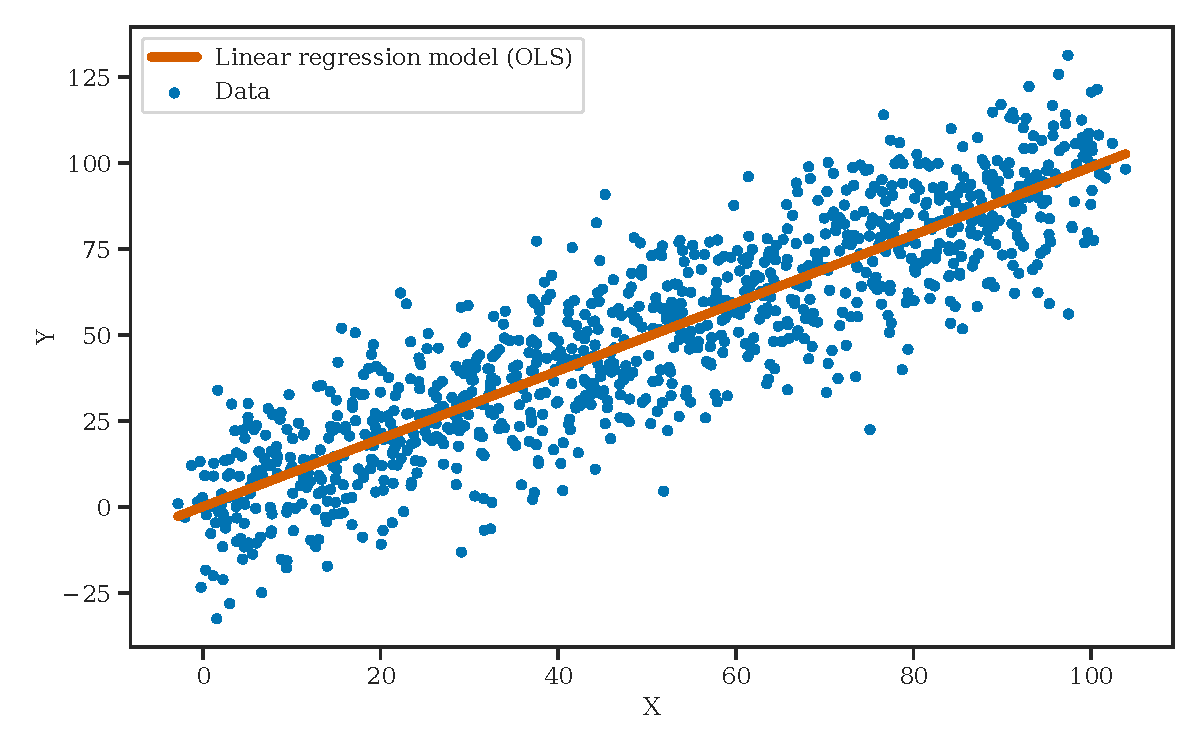
\includegraphics[width=0.8\textwidth]{thesis/figures/linear-regression-example.pdf}
    \caption{Linear regression using OLS, with one dependent variable Y and one independent variable $X$.}
    \label{fig:linear-regression-ols}
\end{figure}

We looked at the simplest form of linear regression, namely only using a single independent variable $X$ to predict a value for $Y$. In order to generalize the linear regression to $k$ independent variables, we now assume that our training data has $k$ variables (also called features, or columns), i.e. $X \in R^{n \times d}$. Finally, we add the new columns from $X$ to the model matrix $X'$, by extending \cref{eqn:y-hat-two-matrix-form} as follows
\begin{align}
    \hat{Y} =
        \undertext{
        \begin{bmatrix}
            1 & x_{11} & \ldots & x_{1k} \\
            1 & x_{21} & \ldots & x_{2k} \\
            \vdots & \vdots & & \vdots \\
            1 & x_{n1} & \ldots & x_{nk} \\
        \end{bmatrix}
        }{$X'$}
        \undertext{
        \begin{bmatrix}
            \hat{\beta}_0 \\
            \hat{\beta}_1 \\
            \vdots \\
            \hat{\beta}_k \\
        \end{bmatrix}
        }{$\hat{\beta}$},
    \label{eqn:y-hat-matrix-form-general}
\end{align}
In order to estimate the model parameters $\hat{\beta}$, we compute them using \cref{eqn:ordinary-least-squares}. Furthermore, we can generalize the minimization objective of OLS (\cref{eqn:RSS-ols-two-variables}) to use $k$ independent variables as well, as seen below:
\begin{align}
    \text{RSS} = \sumlim{i=1}{n}{\enclb{y_i - \enclp{\hat{\beta_0} +  \sumlim{j=1}{k}{\hat{\beta_j}x_{ij}}}}^2}.
    \label{eqn:RSS-ols-k-variables}
\end{align}

\subsection{Lasso regression}
Linear regression suffers from the fact that it has to use all independent variables in order to predict a value for the dependent variable. Imagine that we have gathered some $5$-dimensional data $X$ and want to predict some quantity $y$. We perform some analysis on the data and notice that two of the features of the data is noise and will most likely not help to predict $y$. Lasso regression is a slight modification of linear regression that helps us with this problem. By adding a penalty term on the model parameters in the objective of the linear regression, lasso regression is able to push certain features to 0, essentially "removing" them from the model. If we had two features which were very similar, lasso is also able to "nullify" one of them, since the first one "explains" the second one. As a result, models generated from lasso regression are generally much easier to interpret. What we have described here is also referred to as \textit{feature selection}, where the model automatically selects which variables are useful for prediction.

Lasso regression minimizes the residual sum of squares (RSS) plus some constant $\lambda$ times the $\ell_1$-norm of the model parameters $\beta$, as seen below:
\begin{align}
    \sumlim{i=1}{n}{\enclb{y_i - \enclp{\hat{\beta_0} +  \sumlim{j=1}{k}{\hat{\beta_j}x_{ij}}}}^2} + \lambda ||\beta||_1 = \text{RSS} + \lambda ||\hat{\beta}||_1,
    \label{eqn:lasso-regression-objective}
\end{align}
where $\lambda \geq 0$ is a regularization parameter. The second term of \cref{eqn:lasso-regression-objective}, $\lambda ||\hat{\beta}||_1$, is called the $\ell_1$-penalty and is small when $\hat{\beta}_0$, $\hat{\beta}_1$, \ldots, $\hat{\beta}_k$ are small. When $\lambda = 0$, the penalty term has no effect and lasso regression will produce the same result as standard linear regression. As $\lambda \rightarrow \infty$, the effect of the $\ell_1$-penalty grows and the model parameters $\hat{\beta}$ will approach zero, and in some cases, some of the model parameters will be exactly zero. The $\ell_1$-norm is given by $||\hat{\beta}||_1 = \sum |\hat{\beta}_j|$, where $|\cdot|$ is the absolute value.

\subsection{Logistic regression}
When we described linear regression models in \cref{sec:linear-regression}, we assumed that the response variable $Y$ was quantitative. When working with qualitative data, on the other hand, linear regression fails to work. For example, colors are qualitative, taking on values such as blue, red, green or brown; we can not say that red is greater than blue or brown is less than green (discarding). Predicting a qualitative response variable $Y$ using some data $X$ is also referred to as \textit{classification}. Logistic regression is a method that can predict the response variable $Y$ when it falls into one of two categories (i.e. binary response). Examples of a binary response variable could be "Yes"/"No", "Is a dog"/"Is not a dog" or the typical 0/1 mostly used in machine learning. Logistic regression creates a model that models the probability that $Y$ falls belongs to a particular category. In \cref{fig:logistic-regression-example}, we further motivate the use of logistic regression for binary-response tasks and we see that linear regression is not well suited for predicting values between 0 and 1.
\begin{figure}[H]
    \centering
    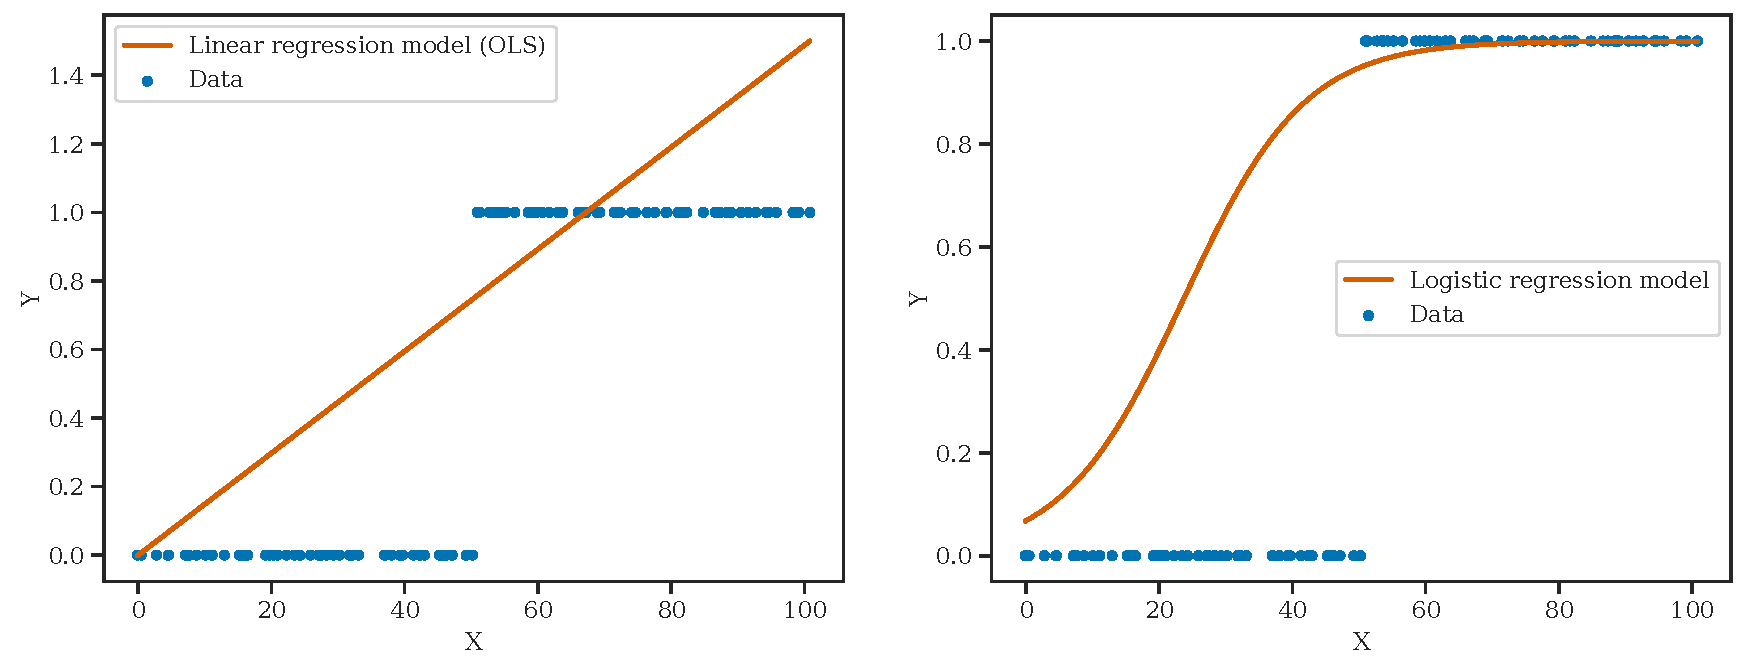
\includegraphics[width=\textwidth]{thesis/figures/logistic-regression-example.pdf}
    \caption{Linear- and logistic regression for predicting some binary response variable $Y$ on data $X$. Here we see that logistic regression is particularly well suited for predicting values for $Y$ between 0 and 1. Linear regression fails to model this relationship, and even goes out of bounds for $X > 70$.}
    \label{fig:logistic-regression-example}
\end{figure}

Let $p(X) = Pr(Y = 1|X)$ denote the probability of $Y$ being 1 given the data $X$. If we want to model this relationship, we could use linear regression by
\begin{align}
    p(X) = \beta_0 + \beta_1 X.
\end{align}
Unfortunately, as mentioned earlier, linear regression is not a good fit for such problems and we would have the situation on the left of \cref{fig:logistic-regression-example}. In logistic regression, the \textit{logistic function} is used to ensure that the output value falls between 0 and 1, as seen below:
\begin{align}
    p(X) = \frac{\exp{\enclp{\beta_0 + \beta_1 X}}}{1 + \exp{\enclp{\beta_0 + \beta_1 X}}}.
    \label{eqn:logistic-function-p-x}
\end{align}
The plot to the right of \cref{fig:logistic-regression-example} shows the effect of the logistic function, creating an S-shaped like curve that for high $X$-values, creates values close to, but never greater than 1. On the other hand, the logistic function creates values close to, but lever less than 0 for low $X$-values. Manipulating \cref{eqn:logistic-function-p-x} a bit, we get that
\begin{align}
    \frac{p(X)}{1 - p(X)} = \exp{\enclp{\beta_0 + \beta_1 X}},
    \label{eqn:logistic-function-odds}
\end{align}
where the left-hand-side of \cref{eqn:logistic-function-odds}, i.e. $p(X)/\enclb{1 - p(X)}$, is called the \textit{odds}. As $p(X)$ increases, the odds increases exponentially towards $\infty$. Taking the logarithm of both sides of \cref{eqn:logistic-function-odds}, we finally arrive at
\begin{align}
    \log \enclp{\frac{p(X)}{1 - p(X)}} = \beta_0 + \beta_1 X,
    \label{eqn:logistic-function-logit}
\end{align}
where the left-hand-side of \cref{eqn:logistic-function-logit} is called the \textit{logit}. Thus, we see that the logistic regression model has a logit that is linear in $X$. If we increase $X$ by one unit, then the log odds is increased by $\beta_1$. However, note that the relationship between $p(X)$ and $X$ in \cref{eqn:logistic-function-p-x} is not a straight line. For this reason, the amount of $p(X)$ changes due to a single unit change in $X$ will depend on the current value of $X$. In \cref{fig:logistic-regression-example}, we see that once $X$ reaches a certain threshold (e.g. $X=30$), the rate at which $Y$ changes decreases towards zero.

If we would like to model logistic regression using multiple predictors, we only have to perform a simple extension from simple to multiple linear regression. We can generalize \cref{eqn:logistic-function-logit} as follows:
\begin{align}
    \log \enclp{\frac{p(X)}{1 - p(X)}}
    &= \beta_0 + \beta_1 X_1 + \beta_2 X_2 + \ldots + \beta_k X_k \\
    &= \beta_0 + \sumlim{i=1}{k}{\beta_i X_i},
    \label{eqn:logistic-function-logit-multiple}
\end{align}
where $X = \enclp{X_1, X_2, \ldots, X_k}$ are $k$ predictors.

In order to estimate the parameters $\beta_0, \beta_1, \ldots, \beta_k$ for $k$ predictors, it is common to use the \textit{maximum likelihood} method. We will not go into detail of the maximum likelihood method here, but kindly refer the reader to \cite[p. 214]{fox2015applied} for more details.

\section{Model selection}
Model selection is a very important aspect of modern machine learning. When working with machine learning, one would like to understand which model fits the use-case at hand the best, and model selection helps us with exactly this. Model selection is the task of selecting a model for a particular problem, given the data at hand. We will look at a couple methods for performing model selection, namely using train/validation/test splits and $K$-fold cross-validation. We refer to \cite{James2013} when describing model selection methods.

\subsection{Train, validation and test splits}
\label{sec:train-val-test-splits}
When training a supervised machine learning model and  we typically have some data $X$ and corresponding labels $y$. The task is to predict the labels $y$ given the data $X$. Since we do not know apriori which model or model parameters to use, the most common way to figure this out is by performing model selection. The simplest kind of model selection for machine learning models is to split the data $X$ and labels $y$ into three data sets, namely the train-, validation-, and test data sets. The new data sets are chosen at random and do not overlap. An example of a train/validation/test split ratio could be 80/10/10, where 80\% of the data is used by the training, 10\% by the validation and 10\% by the test data set. Exactly how we split the data sets into the smaller train/validation/test data sets depends very much so on the application and how much data we are working with. In more modern machine learning models, e.g. using artificual neural networks, it is common to use up to 99\% of the data for training, given that one has a big enough data set (e.g. $>1$ million data points).

The \textit{train data set} is used to learn the models parameters from the data, e.g. a linear regression models $\beta$ parameter. The train data set is usually much larger than the validation or test data sets. In order to evaluate the learned model parameters, the \textit{validation data set} is used. The evaluation of the trained model using a validation data set is also called the \textit{validation set approach}. The validation data set provides an unbiased estimate of a models fit on the training data set while tuning some \textit{hyperparameter}. A hyperparameter is a parameter that we choose for the model beforehand, in contrast to a model parameter, which the model learns internally. Tuning hyperparameters can be a difficult task, especially if one has a lot of hyperparameters with various values. A typical way of performing hyperparameter optimization is by using \textit{grid search}, which tries out all combinations of all hyperparameter values. As grid search can be very computationally expensive if one would like to try out many hyperparameter choices, it is commonly used to find potential ranges where the optimal hyperparameters live.

After selecting a model or a set of model parameters using the validation data set, the \textit{test data set} is used to give an unbiased estimate of how the model performs on unseen data. The test data set is also referred to as the \textit{hold-out data set}, because it is only used at the end of model selection. Note that the test data set is not necessarily needed in order to perform model selection, as it only evaluates the final performance of the final model. A common approach is also to exclude the test data set, and instead split the original data $X$ into training and validation only. By doing so, we are unable to get an unbiased estimate of the models performance on unseen data. We illustrate the process of splitting data into train/validation/test splits in \cref{fig:train-val-test-splits}.
\begin{figure}[H]
    \centering
    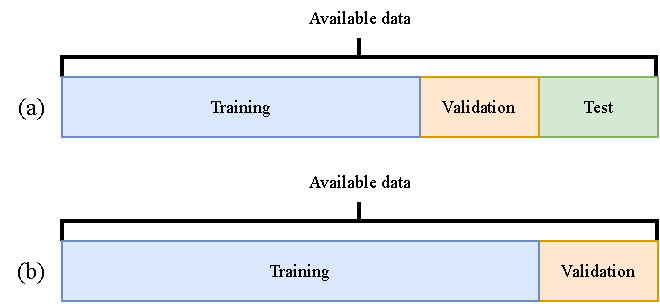
\includegraphics[width=\textwidth]{thesis/figures/train-val-test-splits_cropped.pdf}
    \caption{Example of ways to partition a data set. The partition on the top (a) splits the data into training, validation and test, while the partition on the bottom (b) splits the data into training and validation only.}
    \label{fig:train-val-test-splits}
\end{figure}

The validation set approach is simple and works fine in practice. There are, however, a couple of drawbacks when using this method. Depending on which observations are included in the training- and validation data sets, the validation estimate of the error can vary a lot. In addition to this, since the validation set approach only uses a subset of the observations to train the model and the fact that statistical models perform worse when trained on less data, the validation error rate tend to overestimate the test error rate of a model trained on the entire data set. In the next subsection, we will introduce \textit{$k$-fold cross validation}, an improvement over the validation set approach that addresses these two drawbacks.

\subsection{k-fold cross-validation}
An alternative to the validation set approach is the $k$-fold cross validation (CV) method. The $k$-fold CV method randomly divides the training data $X$ into $k$ groups, or \textit{folds}, of approximately equal size. The first fold is treated as the validation data set and the model is trained on the remaining $(k - 1)$ folds. The first validation error, denoted $\text{Err}_1$ is computed on the validation data set. Following, this procedure is repeated $k$ times, and for each time, a different group of data points from the original training data $X$ is used as the validation data. This results in $k$ estimates of the test error, i.e. $\text{Err}_1$, $\text{Err}_2$, \ldots, $\text{Err}_k$. The total $k$-fold CV error estimate is computed by taking the mean of these values,
\begin{align}
    \text{CV}_k = \frac{1}{k} \sumlim{i=1}{k} \text{Err}_i.
\end{align}
Choosing a value for $k$ is a hard problem. The most common choice is to set $k=5$ or $k=10$, depending on the problem. We kindly refer the reader to \cite[Section 5.1.4]{James2013} for more details on choosing a value for $k$.

An illustrative example of $k$-fold CV is shown in \cref{fig:k-fold-cv}. There we see a typical set up when using a $k$-fold CV, namely to split all available data into training and test data sets. During the training process, the training data set is further more split into training and validation data sets for that particular $k$.
\begin{figure}[H]
    \centering
    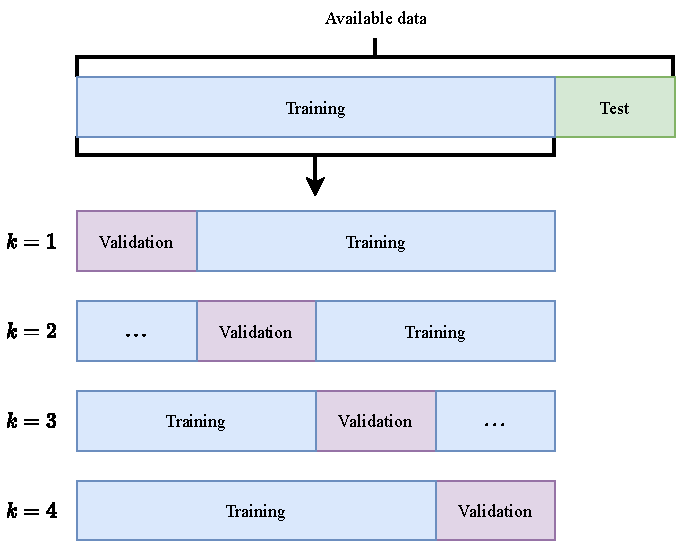
\includegraphics[width=0.9\textwidth]{thesis/figures/k-fold-cv_cropped.pdf}
    \caption{Data split into training and test data sets. In order to perform model selection, $k$-fold cross validation is used. In this example, we have a $4$-fold cross validation setting. As the $k$ increases, we have different data sets for both training and validation.}
    \label{fig:k-fold-cv}
\end{figure}

The benefit of using $k$-fold CV is that, by both training on different subsets of the training data and evaluating the model on different validation data sets, the estimated test error becomes more accurate and we get less varying results, given that we have selected a good value for $k$.

\section{Artificial Neural Networks (ANNs)}
In this section we will explain artificial neural networks (ANN). In particular, we will focus on multilayered neural networks (MLNN). This section is based on \cite[Chapter 1]{Aggarwal18} and \cite{rong2016word2vec}.

An \textit{artificial neuron} (or unit) is a function which receives one or more inputs and a bias, and then sums them to produce an output, as illustrated in \cref{fig:artificial_neuron}; $\left\{ x_1, \ldots, x_K \right\}$ are the input values, $b$ is the bias, $\left\{ w_1, \ldots, w_K \right\}$ are the weights and $y$ is a scalar output. We denote $f$ as the activation function.
\begin{figure}[H]
    \centering
    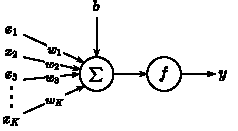
\includegraphics[width=8cm]{thesis/figures/artificial-neuron_cropped.pdf}
    \caption{An artificial neuron taking in a $K$-dimensional input $x$ and bias $b$ to produce some output $y$.}
    \label{fig:artificial_neuron}
\end{figure}

To produce the output of a single unit, we do the following
\begin{align}
    y = f(u)
\end{align}
where $u$ is the input of the neuron. $u$ is defined as
\begin{align}
    u = b + \sumlim{i=1}{K} w_i x_i
\end{align}
which is the weighted sum of the input values $\left\{ x_1, \ldots, x_K \right\}$ plus the bias term, with $\left\{ w_1, \ldots, w_K \right\}$ as weights.

The bias term acts as a intercept value to make the model more general and is usually set to +1. For some models (e.g. word2vec, introduced in \cref{sec:word2vec-as-an-ann}), one does not include the bias term for the units in the neural network, i.e., we leave $b$ to be zero.

The choice of activation function $f$ is typically a non-linear function. Artificial neural networks use different activation functions such as ReLU, sigmoid or tanh to learn non-linear relationships in the data. We will come back to this in \cref{sec:activation-functions-ann}.

\newcommand{\layer}[2]{\left\{ {#1}_{#2} \right\}}

A \textit{layer} $\layer{z}{j} = \left\{ z_1, z_2, \ldots, z_K \right\}$ of an artificial neural network is a collection of artificial neurons (unit). More formally, the layer $\layer{z}{j}$ can be described using an $N \times K$-dimensional weight matrix $W$, a $N$-dimensional bias vector $b$ and an activation function $f$, as seen in \cref{eqn:artificial_layer}.
\begin{align}
    \layer{z}{j} = f \left( W \cdot x + b \right)
    \label{eqn:artificial_layer}
\end{align}
where $x$ is a $K$-dimensional input vector. In the following subsections, we will go over the different types of layers in the ANN, namely the input, hidden and output layers.

\subsection{Input layer}
\label{sec:ann-input-layer}
The first layer in the ANN is the input layer $\layer{x}{k} = \left\{ x_1, x_2, \ldots, x_K \right\}$. It is responsible for taking in input and passing it to the proceeding layer in the network. We illustrate the input layer in \cref{fig:input_layer_ann}.

\begin{figure}[H]
    \centering
    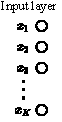
\includegraphics[height=7cm]{thesis/figures/artificial-neural-network-input-layer_cropped.pdf}
    \caption{Input layer in the ANN for a $K$-dimensional vector $x$.}
    \label{fig:input_layer_ann}
\end{figure}

More formally, we define the input layer in \cref{eqn:input_layer_ann} using the definition of a layer. The layer does not perform any changes to the incoming data and acts as a way for feeding data into the neural network. For this reason, \cref{eqn:input_layer_ann} uses the identity matrix $I_K$ as the weight matrix $W_{\layer{x}{k}}$, no bias (i.e. bias equal to zero vector) the identity function $id(x)=x$ as the activation function.
\begin{align}
    \label{eqn:input_layer_ann}
    \layer{x}{k}
    &= f_{\layer{x}{k}}(W_{\layer{x}{k}} \cdot x) \\
    &= id(I_K \cdot x) \\
    &= I_K \cdot x \\
    &= x
\end{align}
With this in mind, we look at the layer the input layer is connected to, namely the hidden layer.

\subsection{Hidden layer}
The hidden layer is the second layer in the ANN $\layer{h}{i} = \left\{ h_1, h_2, \ldots, h_N \right\}$, and is most commonly connected to the input layer. It should be noted, however, that we might have multiple hidden layers in the ANN (making the neural network deeper), connecting them to each other. For illustration purposes, we will assume that we only have one hidden layer in our neural network. The hidden layer is illustrated in \cref{fig:hidden_layer_ann}. Here we observe that every unit in the input layer is connected to the units in the hidden layer, as illustrated the lines. This is what we call fully connected layers, meaning that every unit is connected to each other.

\begin{figure}[H]
    \centering
    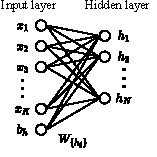
\includegraphics[height=7cm]{thesis/figures/artificial-neural-network-input-hidden-layer_cropped.pdf}
    \caption{Input to hidden layer in the ANN for a $K$-dimensional vector $x$, $N\times K$ dimensional weight matrix $\left\{ W_{h_i} \right\}$ and a $N$-dimensional hidden layer $h$.}
    \label{fig:hidden_layer_ann}
\end{figure}

We formalize the description of the hidden layer in \cref{eqn:hidden-layer-ann}
\begin{align}
    \label{eqn:hidden-layer-ann}
    \layer{h}{i} &= f_{\layer{h}{i}}(W_{\layer{h}{i}} \cdot \layer{x}{k} + b_h)
\end{align}
where $f_{\layer{h}{i}}$ is a user-specified activation function, $W_{\layer{h}{i}}$ is an $N \times K$-dimensional weight matrix and $b_h$ is an $N$-dimensional bias vector.

The hidden layer tries to learn a latent representation of the input data $x$. We will explain how the neural network learns the latent representation when introducing optimizers in \cref{sec:optimizers-ann}. Assuming that we have some $N$-dimensional latent representation of the data, we would like to connect it to the final layer in the neural network, namely the output layer.

\subsection{Output layer}
The last layer in the ANN is the output layer $\layer{y}{j} = \left\{ y_1, y_2, \ldots, y_M \right\}$ and is connected to the last hidden layer. Similar to the hidden layer, we connect each unit in the last hidden layer to each unit in the output layer, as illustrated in \cref{fig:mlnn-one-hidden}.

\begin{figure}[H]
    \centering
    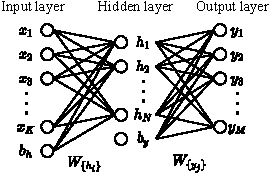
\includegraphics[width=9cm]{thesis/figures/artificial-neural-network_cropped.pdf}
    \caption{Multilayered neural network (MLNN) with one hidden layer.}
    \label{fig:mlnn-one-hidden}
\end{figure}

More formally, we define the output layer $\layer{y}{j}$ using a $M \times N$ weight matrix $W_{\layer{y}{j}}$, an $M$-dimensional bias vector $b_y$ and an activation function $f_{\layer{y}{j}}$, as seen in \cref{eqn:output-layer-ann}.

\begin{align}
    \label{eqn:output-layer-ann}
    \layer{y}{j} &= f_{\layer{y}{j}}(W_{\layer{y}{j}} \cdot \layer{h}{i} + b_y)
\end{align}

We have now covered the different layers in an MLNN, but have yet to cover the different choices of activation function $f$ in the neural network and how the MLNN learns.

\subsection{Activation functions}
\label{sec:activation-functions-ann}
The data which is fed into an ANN might contain complex patterns and have non-linear relationships. To deal with this problem, one applies an activation function to each layer before the result is sent to the proceeding layer. There are several choices of activation functions, and we will go over some of the most common ones.

The simplest type of activation is the identity function, as seen in \cref{eqn:identity-function}.
\begin{align}
    \label{eqn:identity-function}
    f(x) = x
\end{align}

The identity function is commonly used when we want to pass on the values from one layer to another without modifying the value itself, as we have already seen in \cref{sec:ann-input-layer}.

Other choices of activation functions include  sigmoid, tanh, Rectified Linear Unit (ReLU) and softmax, as illustrated in \cref{fig:activation-functions}.
\begin{align}
    \label{eqn:sigmoid-function}
    f(x) &= \frac{1}{1 + \exp{ \left( -x \right) }} \thickspace \text{(sigmoid function)} \\
    \label{eqn:tanh-function}
    f(x) &= \frac{\exp{ \left( 2x \right) } - 1}{\exp{ \left( 2x \right) } + 1} \thickspace \text{(tanh function)} \\
    \label{eqn:relu-function}
    f(x) &= \max{\left\{ x, 0 \right\}} \thickspace \text{(ReLU function)} \\
    \label{eqn:softmax-function}
    f(x_i) &= \frac{\exp \left( x_i \right)}{\sumlim{j=1}{K} \exp \left( x_j \right)} \thickspace \text{, $i \in \left\{ 1, \ldots, K \right\}$ (softmax function)}
\end{align}
where $K$ is the number of output values for the softmax layer.

\begin{figure}[H]
    \centering
    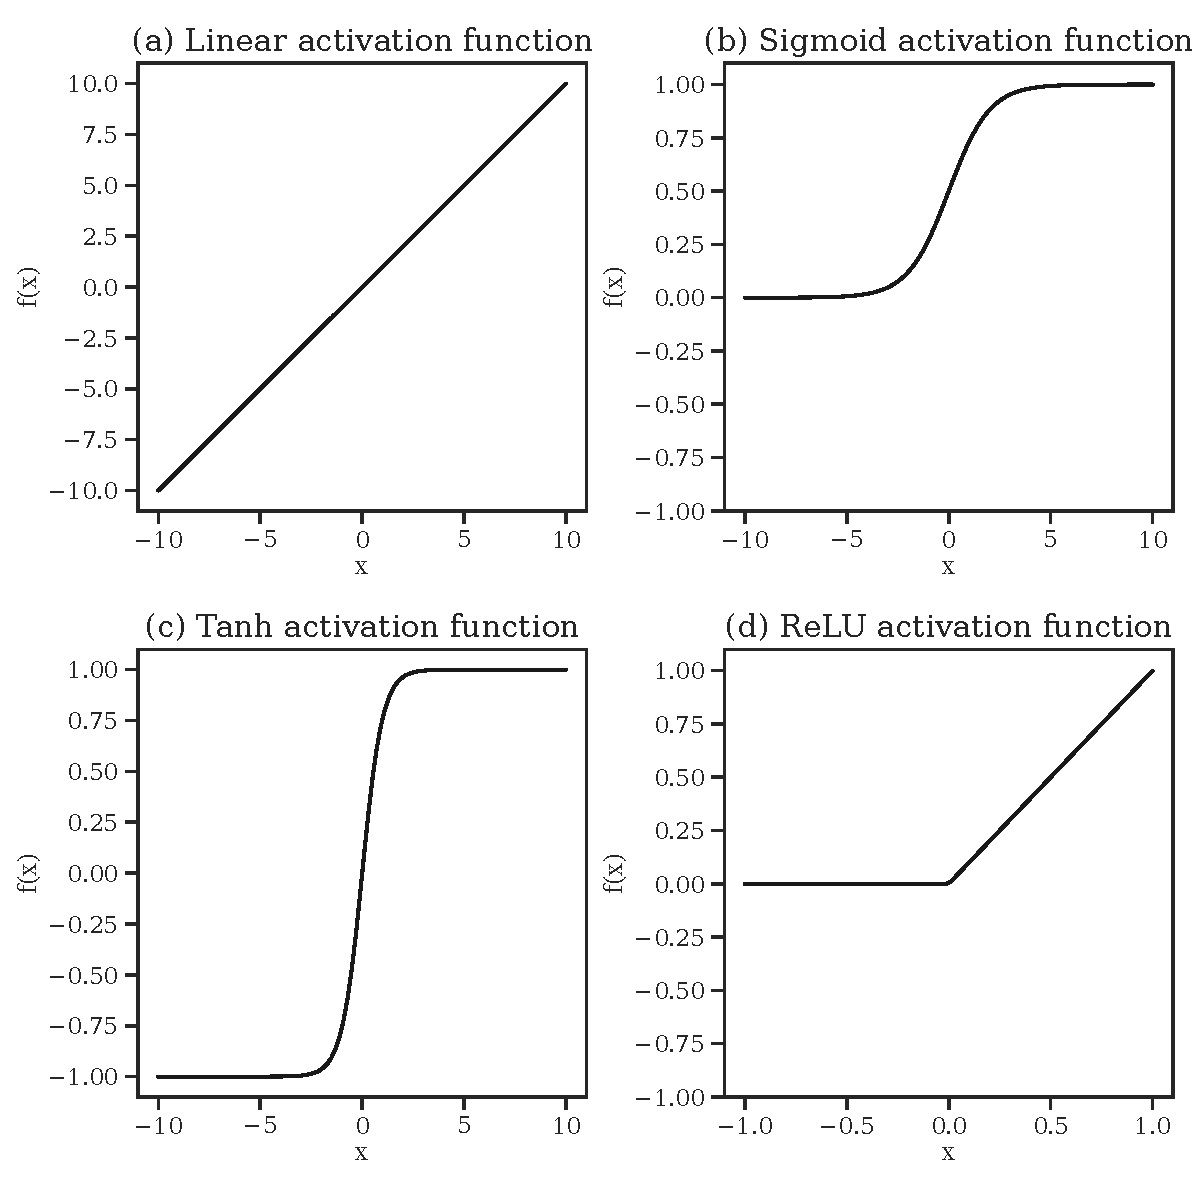
\includegraphics[width=0.7\textwidth]{thesis/figures/common-activation-functions.pdf}
    \caption{Various activation functions}
    \label{fig:activation-functions}
\end{figure}

The sigmoid and tanh activation functions were typically used in the early development of neural networks. The sigmoid activation function maps a value to a value in $(0, 1)$ and is particularly useful since it creates a probabilistic output. The tanh activation function has a similar shape to the sigmoid activation function, and maps values to values in $[-1, 1]$. In fact, the tanh and sigmoid activation functions are related, as illustrated in \cref{eqn:tanh-sigmoid-relation}.
\begin{align}
    \label{eqn:tanh-sigmoid-relation}
    \text{tanh}(x) = 2 \cdot \text{sigmoid}(2x) - 1
\end{align}

In recent years, the ReLU activation function has become more popular, partly due to its computational simplicity. In fact, both the sigmoid and tanh activation function suffers from vanishing gradients (i.e. gradients become zero, leading to very little learning) and ReLU is used as a substitute to overcome this problem. This does not mean, however, that the ReLU activation function can be used without problems, as it can "die out" since it is non-differentiable at 0. We will come back to this problem when introducing the gradient descent optimizer in \cref{sec:optimizers-ann}.

So far we have only discussed activation functions where we have a single output value. If we were to do a classification with $K$ outputs, one typically uses the softmax activation function. The softmax activation function is defined in \cref{eqn:softmax-function} and can be thought of the probabilities of the $K$ outputs.

\subsection{Loss functions}
\label{sec:loss-functions-ann}
So far we have seen how we can connect the different layers in an ANN. In short terms, we are given some input data, send it through some hidden layer and at last get the predicted output values from the output layer. We denote the predicted output values as $\hat{y}$. In this setting, we can assume that we have the true output labels, denoted as $y$. The loss function measures how much the predicted values $\hat{y}$ deviate from the true values $y$, and as such, the goal is to minimize this value. The output layer can have one or many outputs, and depending on the configuration of the network, the loss function changes as well. We separate the output types of an ANN into two categories, namely the regression and classification outputs.

In a regression type output, we usually predict some real-value quantity, such as height, weight or distance. For such problems, it is common to use the mean squared-error (MSE) loss. MSE is calculated as the mean of the squared differences between the predicted and true values, as seen in \cref{eqn:mse}.
\begin{align}
    \label{eqn:mse}
    MSE(\hat{y}, y) = \frac{1}{N} \sumlim{i=1}{N} {\left( y_i - \hat{y_i} \right)}^2
\end{align}
where $N$ is the length of $y$ and $\hat{y}$.

For classification type outputs, we want to classify whether or not some input data belongs to two (binary, e.g., on or off, blue or red) or more classes (categorical, e.g., different types of animals). In a binary classification type output, the sigmoid activation function in conjunction with the binary cross-entropy (BCE) loss function is used. The binary cross-entropy loss function is defined in \cref{eqn:binary-cross-entropy}.
\begin{align}
    \label{eqn:binary-cross-entropy}
    BCE(\hat{y}, y) = -\left( y \cdot \log{\left( \hat{y} \right)} + (1 - y) \cdot \log{\left( 1 - \hat{y} \right)} \right)
\end{align}
As opposed to the binary cross-entropy function, the categorical cross-entropy (CCE) function is used to compute the loss for multi-class classification output. It is common to see the usage of the softmax activation function being used at the output layer to create a multi-class probability distribution. Furthermore, we define the CCE loss function in \cref{eqn:categorical-cross-entropy} and observe that is is simply a generalization of the BCE loss function for multiple classes.
\begin{align}
    \label{eqn:categorical-cross-entropy}
    CCE(\hat{y}, y) = -\sumlim{c=1}{C} y_c \cdot \log{\left( \hat{y_c} \right)}
\end{align}
where $C$ is the number of classes in the multi-class classification output.

\subsection{Optimizers}
\label{sec:optimizers-ann}
In this subsection, we will discuss how an ANN is able to effectively make predictions from input data by learning its internal weights iteratively. In particular, we will look at the gradient descent algorithm and how ANNs exploit it to efficiently perform training.

So far, we have discussed what we call the forward pass (or phase). A forward pass is simply the journey of the input data to the output layers where we in each step compute the output values at each layer and local derivatives using the current set of weights. Once we are at the output layer, the forward pass is complete and the backward pass commences. Recall that the objective of the neural network is to minimize the loss function. To do so, we compute the derivative of the loss function with respect to the weights in the input layer, using the chain rule from calculus. The derivative of the loss function tells the neural network which direction it should move each weight in to minimize the loss (i.e. in the negative direction of the derivative).

To give an example of forward and backward passes in an ANN, consider the example in \cref{fig:neural-network-example-backprop}.
\begin{figure}[H]
    \centering
    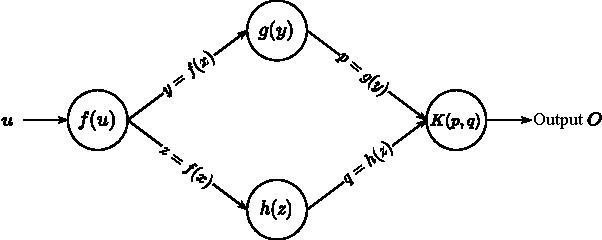
\includegraphics[width=12cm]{thesis/figures/artificial-neural-network-backprop-example_cropped.pdf}
    \caption{Neural network with one input node, one hidden layer with two nodes and a single output layer.}
    \label{fig:neural-network-example-backprop}
\end{figure}

In this example, we are given a network with one input node (neuron), a hidden layer with two nodes and a single output layer with one node. The input to the network is denoted as $u$ and is the product of the input data and the weights in the input layer. The activation functions of the network are denoted as $f$, $g$ and $h$. Moreover, the results of the activation functions are denoted as $y$, $z$, $p$, $q$, and the function $K$ combines the result of $p$ and $q$ resulting in the output value $O$. We assume that the weights of the hidden layer is applied to the previous layer's output values during $g$ and $h$ and the weights of the output layer is applied at $K$. The forward pass in this network is pretty straight forward; we start the input node, pass the data on to $g$ and $h$ and combine the results in the output layer. Now, for the backwards pass we first need to compute the loss at the output node using a loss function $L$. Furthermore, we compute the derivative of $L$ with respect to the input $u$. More formally, we need to compute
\begin{align}
    \parder{L}{u}
    &= \parder{L}{O} \cdot \parder{O}{u} \\
    &= \parder{L}{O} \cdot \left[
    \parder{O}{p} \cdot \parder{p}{u} +
    \parder{O}{q} \cdot \parder{q}{u}
    \right] \text{(chain rule)} \\
    &= \parder{L}{O} \cdot \left[
    \parder{O}{p} \cdot \parder{p}{y} \cdot \parder{y}{u} + 
    \parder{O}{q} \cdot \parder{q}{z} \cdot \parder{z}{u}
    \right] \text{(chain rule)} \\
    &= \parder{L}{O} \cdot \left[
    \undertext{\parder{K(p, q)}{p} \cdot g'(y) \cdot f'(u)}{Path on top} + 
    \undertext{\parder{K(p, q)}{q} \cdot h'(z) \cdot f'(u)}{Path on bottom}
    \right]
\end{align}

With this example in mind, we have illustrated how the derivatives are being calculated for a small neural network. There exists, effective and more general frameworks to derive the derivative of the loss with respect to the input values, but we will leave those details out and kindly refer the reader to \cite[Chapter 1.3]{Aggarwal18} for more details.

We have now gone over the forward and backward passes, which are the first two steps of the so called backpropagation algorithm. The remaining step of the algorithm is now to use the computed derivatives to update the weights of the ANN. To do this, we use the gradient descent (GD) algorithm. The main idea of gradient descent is to update the weights iteratively by moving them in the opposite direction of the gradient (i.e. the steepest descent), and by doing so, we will hopefully reach some local minimum leading better to fitting weights for the input-output data. In standard gradient descent, we perform its steps in the following manner
\begin{align}
    W \Leftarrow W - \alpha \cdot \parder{L}{W}
\end{align}
where $W = \left( w_1, w_2, \ldots, w_d \right)$ is the matrix consisting of the $d$ weights of an ANN. The learning rate $\alpha$ is a hyperparameter and determines how much learning we want to do in each step. The learning rate is usually set to a relatively low value, in the order of $10^{-2}$ to $10^{-5}$.

Even though gradient descent works great for small applications, once we scale the number of parameters (weights) in the ANN to the more extremes (e.g. in the order of millions), it becomes impractical to compute for the entire training data at once. Furthermore, we observe that a loss function $L$ usually can be written as a sum of the loss of the individual training data points (denoted $L_i$ for $i$th training point), as shown in \cref{eqn:loss-function-sum-individual}.
\begin{align}
    \label{eqn:loss-function-sum-individual}
    L = \sumlim{i=1}{n} L_i
\end{align}
Using the observation that we are able to write the loss function as the sum in \cref{eqn:loss-function-sum-individual}, we introduce the stochastic gradient descent (SGD) method. Instead of performing gradient descent on the whole input data, SGD instead performs gradient descent for each input data separately, as shown in \cref{eqn:sgd}. We call it stochastic, because a random sample of the training data is chosen for each iteration.
\begin{align}
    \label{eqn:sgd}
    W \Leftarrow W - \alpha \cdot \parder{L_i}{W}
\end{align}
where $n$ is the number of input data points and $L_i$ represents the loss the $i$th input. An advantage SGD has over GD, is that it runs a lot faster, at the expense of greater loss. Thankfully, there exists a variant of SGD which seeks to find a balance between speed and loss, namely the mini-batch stochastic gradient descent. In mini-batch stochastic gradient descent, one uses a batch $B=\enclc{j_1, \ldots, j_m}$ of input training data indices when computing the weight updating, as shown in \cref{eqn:mbsgd}.
\begin{align}
    \label{eqn:mbsgd}
    W \Leftarrow W - \alpha \cdot \sumlim{j \in B}{} \parder{L_j}{W}
\end{align}
Mini-batch stochastic gradient descent often finds the best trade-off between stability, speed and memory requirements. It should be noted, however, that the memory requirement increases with the use of mini-batches, due to the fact that we have to store bigger matrices in memory during training. One typically chooses batch sizes that are power of 2 (e.g. 32, 64, 128 or 256), since most modern hardware architectures are optimized for it.

In addition to the different variants of gradient descent, there exist a bunch of other variants which can solve issues such as getting stuck in local minimas or speeding up the training process. We will not go into detail on all these strategies here, but kindly refer the reader to \cite[Chapter 3.5]{Aggarwal18} for more details.

\section{Clustering algorithms}
\label{sec:clustering-algorithms}
In a supervised machine learning setting, we usually are given some data $X$ and associated labels $y$. The supervised task is to train a model to predict the labels $y$ given data $X$. A classical example of a supervised machine learning task is to distinguish between dogs and cats, where $X$ is an image of the dogs and cats and the labels $y$ indicate whether or not the data $X$ represents a dog ($y=0$) or a cat ($y=1$). In an unsupervised setting, however, the labels $y$ might not be present. To predict the labels $y$, clustering algorithms are usually applied.

Clustering is one of the most important methods in unsupervised machine learning. Clustering algorithms divides some data $X$ into clusters (groups) such that the data in each cluster are similar in some sense. An example of this is clustering by distance (e.g. Euclidean). If we cluster by distance, we want the distance between any two data points belonging to the same cluster to be small. This distance is also referred to as the intracluster distance or compactness. Unfortunately, it is usually not enough to only minimize the intracluster distance, we also have to ensure that distance between the clusters is as large as possible. To measure the distance the distance between two clusters we measure the distance between two data points belonging to different clusters. The distance between clusters is called the intercluster distance or separation. If a clustering algorithm is able to create clusters such that we have small intracluster distance and large intercluster distance, it indicates that the cluster algorithm is good for the data at hand. We note, however, that data can be very complex and it can be very hard to find good clusters.

We will now go over some common clustering algorithms, explain how they work and discuss their strengths/weaknesses. In each of the clustering algorithms, we can assume that we are given some data $X = \enclc{x_1, x_2, \ldots, x_n} \in \R^{n \times d}$.

\subsection{k-means clustering}
\label{sec:k-means-clustering}
The k-means clustering method \cite[Section 9.1]{bishop2006} is an unsupervised machine learning algorithm used to identify clusters in data. The algorithm uses an iterative approach to search for $k$ clusters, where $k$ is a pre-determined number of clusters (i.e. hyperparameter). There exists several variants of this algorithm and we will discuss two of them in later subsections (\cref{sec:mini-batch-k-means-clustering} and \cref{sec:k-medoids-clustering}). We will now explain the standard (and naïve) variant of the algorithm, usually referred to as Lloyd's algorithm, and we base this section on \cite[Section 9.1]{bishop2006}.

The standard k-means clustering algorithm works as follows. The first step is to determine the initial cluster means, or centroids. Since we want the algorithm to output $k$ clusters, we have to decide $k$ initial centroids. The simplest way to do this is to select $k$ random data points to be the initial $k$ centroids. The next step is to calculate the Euclidean distance between each data point to the cluster centroids. We do so because we want to determine which cluster each data point belong to. Furthermore, we assign each data point to its closest cluster centroid and compute the mean of each cluster. The third and final step is to move the cluster centroid to the newly computed mean of each cluster. The second and third step is then repeated until the desired clustering is achieved.

More formally, the goal of k-means clustering is to minimize the squared distance between the points in each cluster to its respective centroid. This is also referred to as the within-cluster sum of squares (WCSS). The objective is to find
\begin{align}
    \argmin_{C} \sumlim{i=1}{k} \sumlim{x \in C_i}{} \norm{x - \mu_i}^2
\end{align}
where $C = \enclc{C_1, C_2, \ldots, C_k}$ are the clusters of the data $X$, $k$ is the desired number of clusters and $\mu_i$ is the cluster centroid of cluster $C_i$.

The main advantage of k-means clustering is its simplicity, both in implementation and interpreting the results. The algorithm also scales well to larger data sets and there is only one hyperparameter to tune (number of clusters $k$). As for the disadvantages, the algorithm is rather sensitive to the initialization of centroids in the first step. If we were to select very bad initial centroids, the convergence time of the algorithm increases greatly and we might not even get good clusters. We also have to choose the number of clusters manually, which is a downside if we have no additional knowledge of the data beforehand. In addition to this, the algorithm (as with any distance-based clustering algorithm) suffers from the curse of dimensionality (\cref{fig:curse-of-dimensionality}), i.e., the fact that when the dimensionality increases it becomes more and more difficult to distinguish between data points (all points converge to the same distance).

\begin{figure}[H]
    \centering
    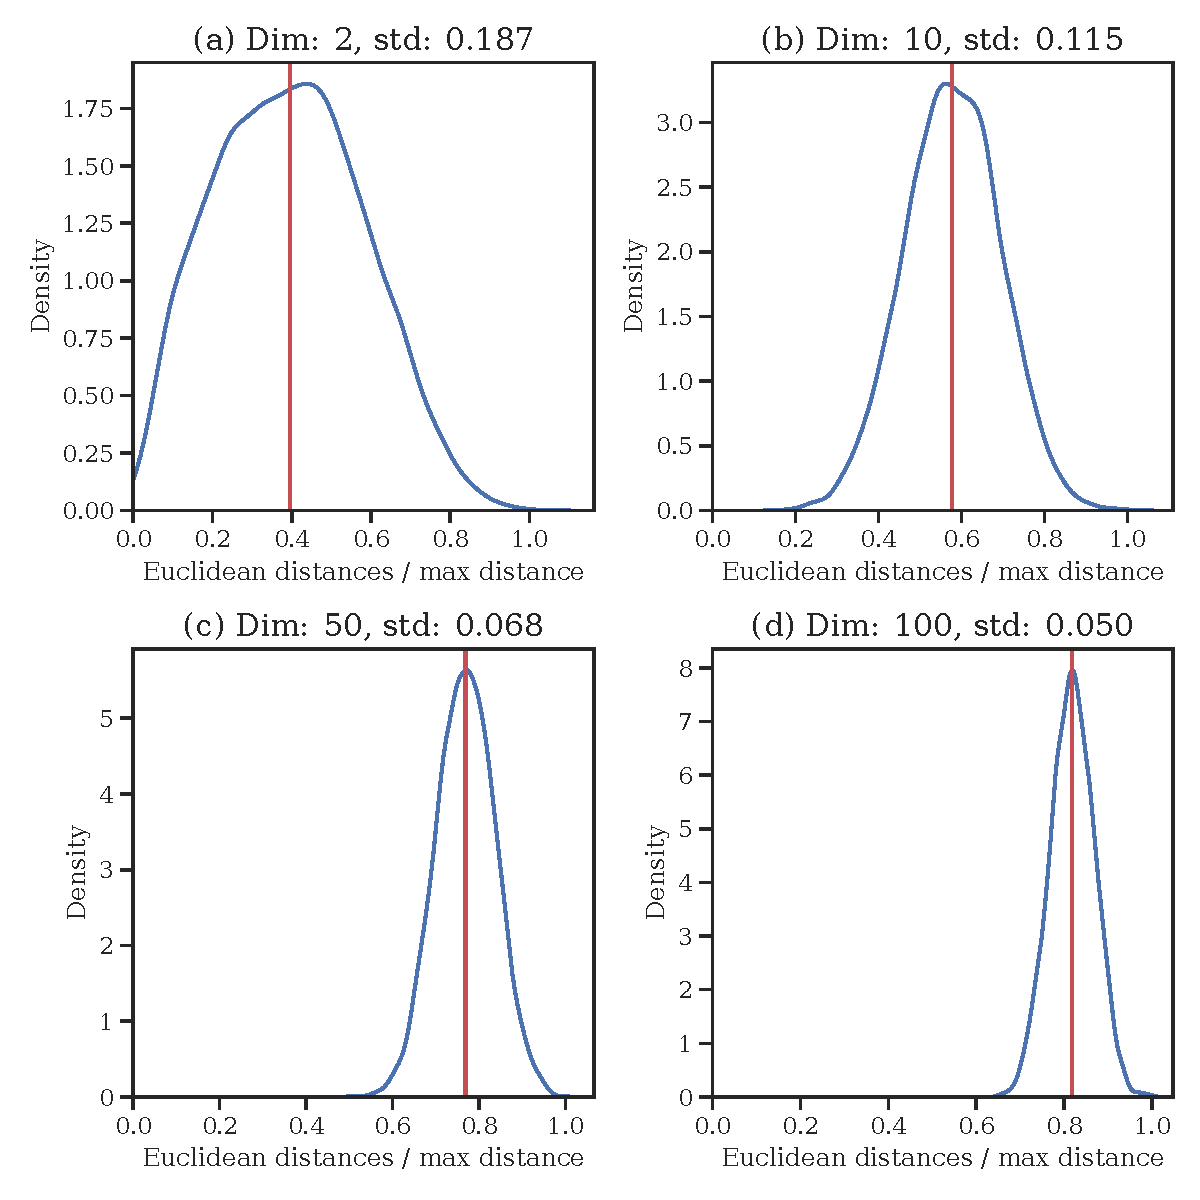
\includegraphics[width=0.7\textwidth]{thesis/figures/curse-of-dimensionality.pdf}
    \caption{Curse of dimensionality: the distance between points in higher dimensional spaces become the same as the dimensionality increases, and thus, it is harder to differentiate between points using distance metrics. The blue line represents the density of the pairwise Euclidean distances (divided by max distance to normalize x-axis). The red line is the mean distance.}
    \label{fig:curse-of-dimensionality}
\end{figure}

\subsection{Mini-batch k-means clustering}
\label{sec:mini-batch-k-means-clustering}
Mini-batch k-means clustering is a variant of k-means clustering, where mini-batches of data points are used in order to find a suitable clustering \cite{sculley2010}. The mini-batches are randomly sampled subsets of the training data for each training iteration (similar to the mini-batches in gradient descent). We refer to \cite{sculley2010} when explaining mini-batch k-means clustering.

The algorithm is very similar to the standard k-means clustering algorithm and comprises two major steps. In the first step, we initialize $k$ cluster centroids and sample $B=\enclc{b_1, b_2, \ldots, b_m} \subset X$ points at random from the data set $X$, where $m$ is the mini-batch size. In the second step, we update the cluster centroids by gradually moving the centroids. For each sample $b$ in the mini-batch, the centroids are updated by taking the average of $b$ and the previous points assigned to the centroid. By doing so, the centroid is moved with a decreasing rate over time. The first and the second step is repeated until convergence is met.

The main advantage of mini-batch k-means clustering over standard k-means, is that the convergence time is lower. By using mini-batches, we drastically reduce the computational requirement required to converge to a local solution and, as noted by the authors in \cite{sculley2010}, the results of mini-batch k-means clustering tend to only be slightly worse than the standard algorithm.

\subsection{k-medoids clustering}
\label{sec:k-medoids-clustering}
K-medoids clustering was introduced as an alternative to the standard k-means clustering algorithm \cites{Kaufman1990}[p. 427 - 428]{bishop2006}. K-medoids clustering uses data points for its cluster centroids and works with any dissimilarity measures. A medoid of a cluster is a data point where the average dissimilarity between the medoid itself and all other data points in the same cluster is being minimized \cite{Kaufman1990}. We refer to \cites{Kaufman1990}[p. 427 - 428]{bishop2006}\, when explaining k-medoids clustering.

To solve the k-medoids problem efficiently, the Partitioning Around Medoids (PAM) algorithm is often used. Similar to the standard k-means clustering algorithm, PAM consists of two main stages called build and swap. In the build stage, we greedily select $k$ of the $n$ data points to be the initial cluster medoids, denoted $M = \enclc{m_1, m_2, \ldots, m_k} \subset X$. To select $M$ initially, we want to minimize the dissimilarity between the cluster medoids and associated points in the cluster. In other words, initially we set the first medoid $m_1$ to be the data point such that the dissimilarity between then medoid and all other data points is minimized. Then, for all proceeding medoids ($m_2, \ldots, m_k$), we look for medoids such that the dissimilarity between the additional medoid, the data points associated with the new medoid and all other medoids (and its associated data points) is minimized. This process is repeated until we have $k$ medoids. Following, the swap stage consists of iteratively swapping out the $k$ medoids with other data points from the data set, if it minimizes the overall dissimilarity. The algorithm terminates if by swapping the medoids with other data points we do not get lower dissimilarity.

The main advantage of k-medoids is that it is more interpretable and robust to outliers than the standard k-means clustering algorithm, since it uses actual data points as centroids. In addition to this, any dissimilarity measure can be used, whereas in standard k-means clustering Euclidean distance is the only option. Even though k-medoids clustering seems to be the superior choice over k-means clustering, it suffers from the fact it is more computationally heavy to compute and thus is not always feasible to run for large data sets.

\subsection{Gaussian mixture models (GMMs)}
\label{sec:gmm-clustering}
Gaussian mixture models (GMMs) are probability distributions which consists of a mixture of multiple Gaussians \cite[Section 9.2]{bishop2006}. A Gaussian (also called normal) is a probability distribution which was several nice properties, such as mean as its mode and symmetry. In the context of cluster algorithms, GMMs can be used to cluster data points by using multivariate (i.e. of higher dimension) Gaussian distributions as cluster centroids. In particular, for each cluster centroid $c_i, 1 \leq i \leq k$, we define $\mu_i$ to be the cluster mean, $\Sigma_i$ to be the cluster covariances and $\pi_i$ to be the mixing coefficients. The cluster mean $\mu_i$ and covariances $\Sigma_i$ determines the localization and spread for each cluster, while the mixing coefficients $\pi_i$ determine how much we emphasize each cluster. To estimate the parameters $\theta = \enclc{\mu, \Sigma, \pi}$ of GMMs, the Expectation-Maximization (EM) algorithm is often used and is an iterative algorithm. When explaining GMMs and the EM algorithm, we refer to \cite[Section 9.2]{bishop2006}.

The EM algorithm starts off my initializing its parameters $\mu$, $\Sigma$ and $\pi$. There exists several methods for initializing the parameters and it is common to first run k-means clustering on the data in order to obtain a suitable starting point. By running k-means clustering first, the parameters are computed by using statistics from the result of k-means. Furthermore, the EM algorithm consists of two main stages, namely expectation and maximization. In the expectation stage we compute the responsibilities for each data point in $X$ using the current set of parameters. With responsibilities, we mean how much each Gaussian is responsible for explaining a single data point in $X$. Next, in the maximization step, the responsibilities from the expectation step is used to update the parameters such that the likelihood $\text{P}(X | \theta)$ is maximized. The likelihood $\text{P}(X | \theta)$ tells us how good the set of parameters $\theta$ fits our data $X$. The exact derivation and update rules for each parameter is left out and we refer the reader to \cite[Section 9.4]{bishop2006} for more details. Once a suitable threshold is met with respect to $\text{P}(X | \theta)$, the algorithm terminates and we have converged to a set or parameters $\hat{\theta}$. Using the final parameters, $\hat{\theta}$ we predict which Gaussian (i.e. cluster) each data point in $X$ is associated with.

The main advantage of using GMMs is that clusters can be differently shaped and we get a probabilistic measure of which cluster each data point belong to (i.e. fuzzy clustering). The convergence time of GMMs depends on the initialization of the parameters $\theta$. If k-means clustering is first used to initialize the parameters, then the overall convergence time is greater than simply running k-means alone. If a completely random initialization of the $\theta$ is used, then it converges a lot faster at the risk of converging in a bad local maxima, leading to worse results.

\subsection{Hierarchical clustering}
\label{sec:hierarhical-clustering}
Hierarchical clustering is a group of clustering algorithms which constructs clusters by recursively partitioning the data points of $X$ in top-down or bottom-up fashion \cite{Rokach2005}. These two methods are divided into what we call agglomerative- and divisive hierarchical clustering. This section is based on \cite{Rokach2005}.

Using the agglomerative hierarchical clustering, each data point in $X$ starts off in their own cluster and are successively merged until all points are merged into a single cluster. In contrast to the agglomerative method, divisive hierarchical clustering starts off with all data points in $X$ in a single cluster. Then, the single cluster is divided into smaller clusters, until each point is in its own cluster. The output of an hierarchical clustering algorithm is a dendrogram, which represents the nested clustering structure. An example of a dendrogram is illustrated in \cref{fig:dendrogram-example}.
\begin{figure}[H]
    \centering
    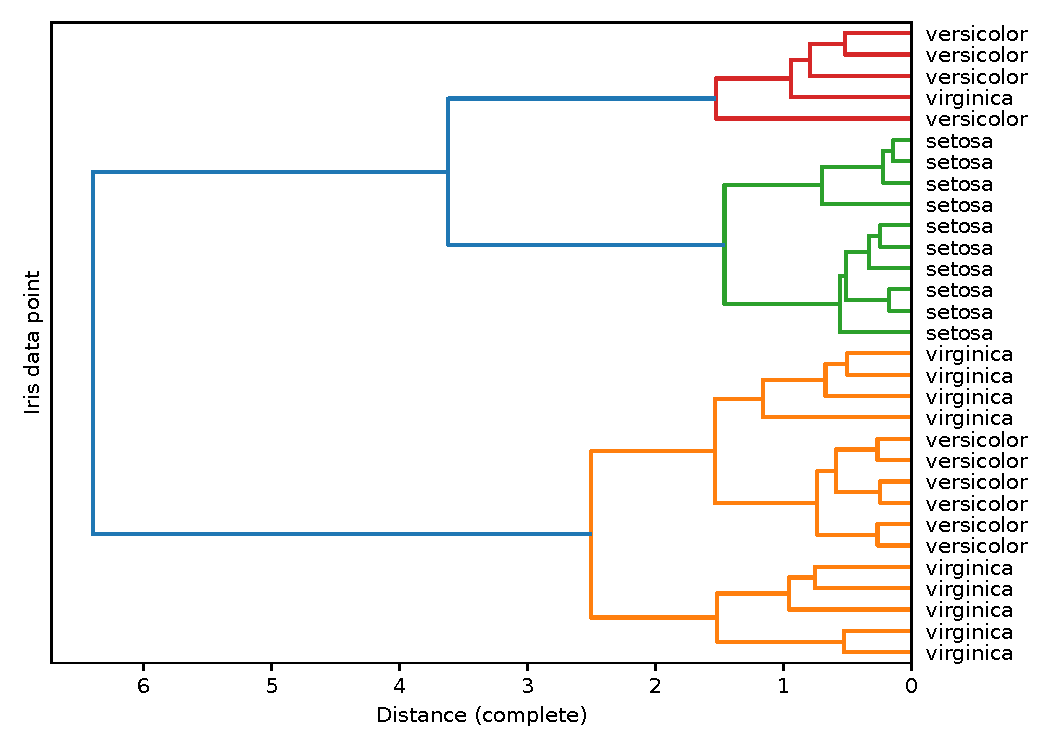
\includegraphics[width=0.9\textwidth]{thesis/figures/dendrogram-example.pdf}
    \caption{Example of a dendrogram plot using the Iris data set \cite{Fisher1936}.}
    \label{fig:dendrogram-example}
\end{figure}

To merge or divide clusters, we use some similarity measure in order to either merge similar data points (agglomerative) or divide dissimilar data points (divisive). Exactly which data points we choose to merge or divide depends on which criterion we want to optimize. There exist several different criterions one may choose to perform hierarchical clustering. Below we will list some of the most common ones and mention some pros/cons for each criterion.
\begin{itemize}
    \item \textbf{Single-linkage clustering} --- combines two clusters that contain the closest pair (i.e. largest similarity) of elements that do not yet belong to the same cluster as each other.
    \begin{itemize}
        \item Single-linkage clustering tends to produce clusters of long chains, which can lead to the clustering of data points which in reality are far apart from each other.
        \item Single-linkage clustering is fast to use for big data sets and is able to create clusters of different shapes and sizes.
        \item Single-linkage clustering is sensible to noise.
    \end{itemize}
    \item \textbf{Complete-linkage clustering}  --- combines two clusters that contain the furthest pair (i.e. smallest similarity) of elements that do not yet belong to the same cluster as each other.
    \begin{itemize}
        \item Complete-linkage clustering is biased towards spherical clusters.
        \item Complete-linkage clustering works well on data with noise.
        \item Complete-linkage clustering tends to split large clusters.
    \end{itemize}
    \item \textbf{Average-linkage clustering} --- combines two clusters such that the average pairwise distance within the newly created cluster is minimum.
    \begin{itemize}
        \item Average-linkage clustering is biased towards spherical clusters.
        \item Average-linkage clustering works well on data with noise.
    \end{itemize}
    \item \textbf{Ward-linkage clustering} --- combines two clusters such that the variance of the newly created cluster is minimum \cite{Ward1963}.
    \begin{itemize}
        \item Ward-linkage clustering is biased towards spherical clusters.
        \item Ward-linkage clustering works well on data with noise.
    \end{itemize}
\end{itemize}

Overall, hierarchical clustering is a great clustering algorithm for partitioning the data in a tree-fashion. By performing hierarchical clustering, we can use the resulting dendrogram in order to determine the number of clusters by cutting it at a certain distance threshold. In the example from \cref{fig:dendrogram-example}, a suitable cut could be at distance equal to 3, leading to 3 clusters. In addition to this, different choices of linkages can lead to very different clusterings. For this reason, one should test multiple linkages to figure out what fits the data the most.

\subsection{Spectral clustering}
\label{sec:spectral-clustering}
Spectral clustering is a clustering algorithm which first, reduces the dimensionality of the data set and then applies a clustering algorithm \cite{Andrew2002}. In particular, spectral clustering uses the eigenvalues of the affinity matrix (e.g. a similarity matrix using pairwise Euclidean distances) of the data $X$ to reduce the dimensionality of the data, before applying some common clustering algorithm, such as k-means clustering. This section is based on \cite{Andrew2002}.

Imagine that we want to cluster the data into $k$ clusters. Spectral clustering starts off with the construction of the affinity matrix $A$. Typically, one uses some similarity measure to create pairwise distances between data points to create such an affinity matrix. Then, the graph Laplacian $L = D - A$ is computed, where $D$ is a diagonal matrix with $D_{ii} = \sumlim{j}{} A_{ij}$ and $A$ is the affinity matrix. The graph Laplacian $L$ is simply a matrix representation of a graph, and in our case, the similarities between data points in $X$. Next, the eigenvectors of $L$ is computed, and using these eigenvectors, we now have a lower-dimensional space of the original data $X$ (from $d$ dimensions to $k$). Lastly, we use a clustering algorithm, such as k-means clustering, on the eigenvectors of $L$ to get the final clustering.

The main advantage of spectral clustering is that it performs a dimensionality reduction on the data, before apply a clustering algorithm. The dimensionality reduction can make the clustering algorithm less prone to noise and yield better results. Unfortunately, the computational requirement of spectral clustering is rather high, and for big data sets it is simply infeasible.

\subsection{HDBSCAN}
\label{sec:hdbscan-clustering}
Clusters come in different shapes and sizes, and real-life data is rather noisy. DBSCAN is a density-based algorithm invented to cope with such problems \cite{Ester1996}. It, however, is only able to produce a "flat" clustering given some global threshold parameter. HDBSCAN is a generalization of DBSCAN and improves on it by creating a complete density-based clustering hierarchy \cite{Campello2013}, automatically extracting flat clusters. HDBSCAN is different from the other clustering algorithms we have seen so far, as it is able to create clustering without predetermining the number of clusters beforehand and can mark data points a noise. To fully understand the HDBSCAN algorithm, we will introduce its key concepts and then explain how the algorithm works in practice. This section is based on the "How HDBSCAN Works" article from \cite{how-hdbscan-works-2016}.

HDBSCAN is a density-based clustering algorithm and, for this reason, requires an inexpensive density estimation method to be efficient. Using k-nearest neighbours, the authors of HDBSCAN is able to estimate the density in an efficient manner. In particular, they define the \textbf{core distance} of a data point $x \in X$ to be the distance to the $\textit{minPts}$-nearest neighbour (including $x$), denoted $d_{core}(x)$. $\textit{minPts}$ is a hyperparameter and controls how conservative we want the clustering to be; the larger $\textit{minPts}$, the more points will be marked as "noise". To further spread apart data points that have low density, the \textbf{mutual reachability distance} metric (MRD) is defined, as seen in \cref{eqn:mutual_reachability_distance}.
\begin{align}
    d_{mreach}(x, y) = \max \enclc{ d_{core}(x), d_{core}(y), d(x, y) }
    \label{eqn:mutual_reachability_distance}
\end{align}
where $d(x, y)$ is the distance between data point $x$ and data point $y$ using the original distance metric. Under the MRD metric, data points in dense regions will not change their distances, but sparser data points will be pushed away such that the distance is at least their core distance to other points.

Next, given the MRD metric, we use it to find dense areas in the data. To find such areas, we create a minimal spanning tree (MST) where each node represents a data point $x \in X$ and edges connecting pairs of nodes is weighted by the MRD between the two nodes. By using an MST, we get a graph with the minimal set of edges between nodes such that the weight between the nodes is minimized. Also, by dropping one edge, we graph becomes disconnected, i.e., each pair of nodes is connected by exactly one edge. Using these two facts, we can create a clustering hierarchy in a single-linkage clustering manner. First, the weights of the edges of the MST is sorted in increasing order. Following, we iterate over the sorted edges of the MST and merge data points into clusters (note that each individual data point is its own cluster initially). Now, from the hierarchical clustering we are left with a dendrogram, as illustrated in \cref{fig:hdbscan-dendrogram-example}, but are left with a critical question; how should we define the cut in order to get a flat clustering?
\begin{figure}[H]
    \centering
    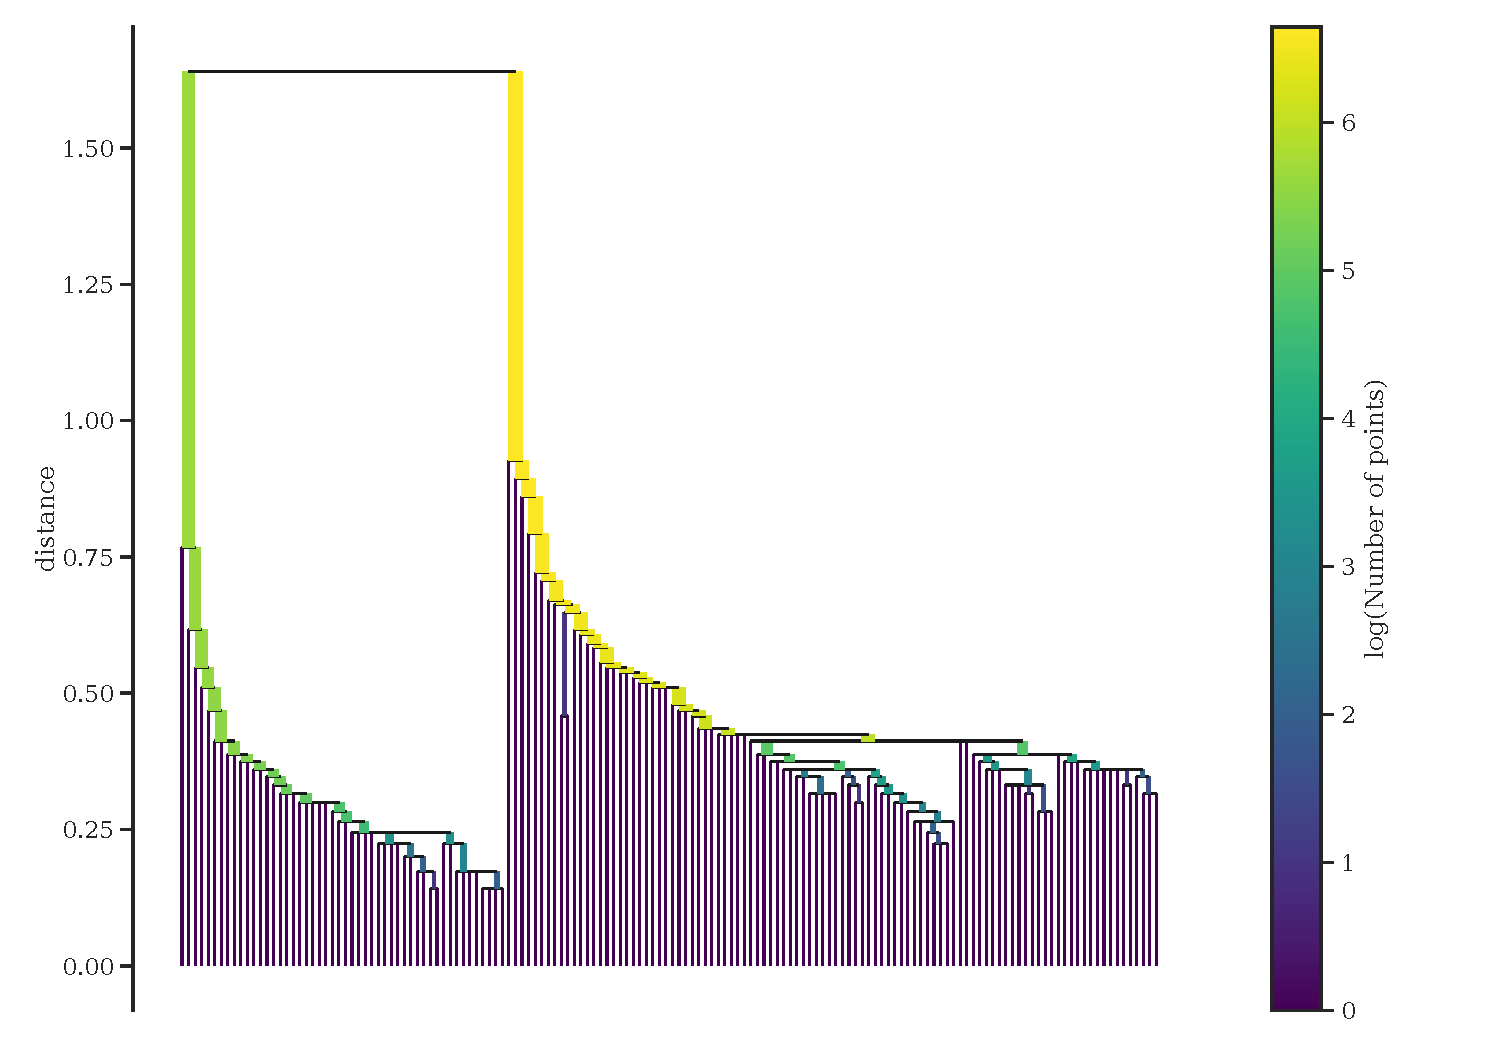
\includegraphics[width=10cm]{thesis/figures/hdbscan-single-linage-tree-example.pdf}
    \caption{Single-linkage dendrogram plot from HDBSCAN on the Iris data set \cite{Fisher1936}.}
    \label{fig:hdbscan-dendrogram-example}
\end{figure}

Dendrograms can be very difficult to interpret once a certain number of data points is reached. For this reason, the authors of HDBSCAN condense (or compact) the dendrogram from the hierarchical clustering such that a flat clustering can be obtained rather easily. First, the notion of \textbf{minimum cluster size} is defined and is a hyperparameter controlling the minimal cluster size at any time. Following, we walk down the dendrogram, starting from the root cluster, and at each split we check whether or not the new cluster created by the split has at least \textbf{minimum cluster size} data points in them. If the new cluster has at least \textbf{minimum cluster size} data points in them, we let that cluster be in the tree. If the new cluster has less than the \textbf{minimum cluster size}, then we let the parent cluster identify the new cluster and the node is removed from the tree. As we walk through the dendrogram in order to condense it, we also include at what distance clusters merge into the parent cluster, i.e., "fall out of clusters". An example of a condensed diagram is down in \cref{fig:hdbscan-condensed-dendrogram-example}.
\begin{figure}[H]
    \centering
    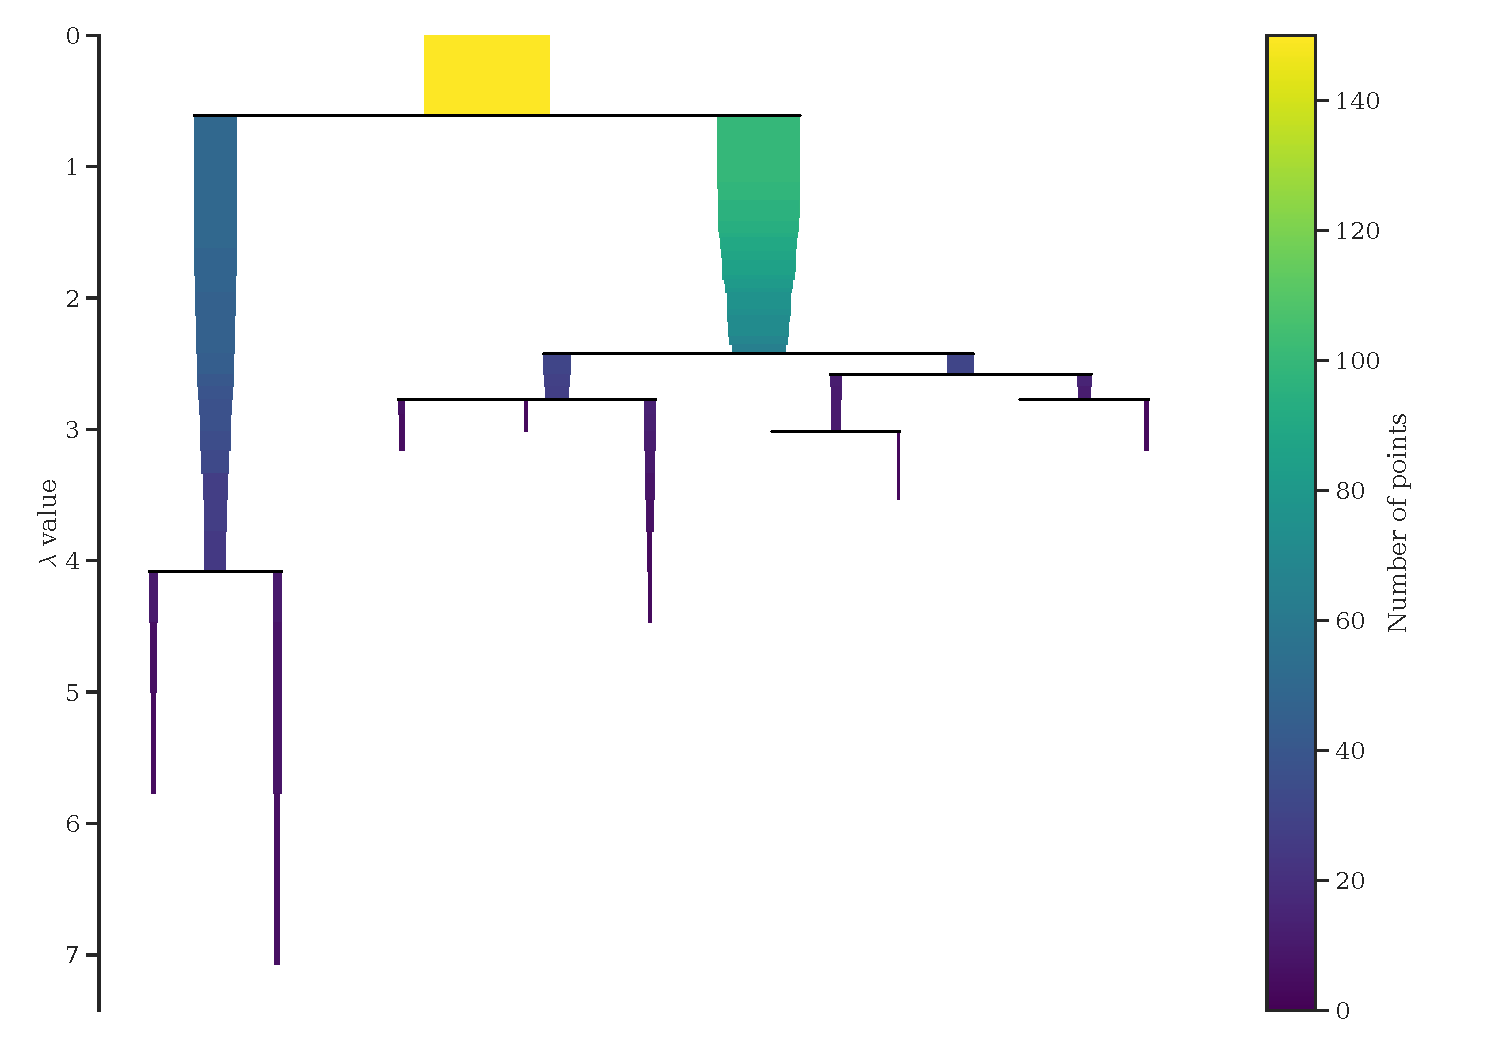
\includegraphics[width=10cm]{thesis/figures/hdbscan-condensed-tree-example.pdf}
    \caption{Condensed dendrogram plot from HDBSCAN on the Iris data set \cite{Fisher1936}.}
    \label{fig:hdbscan-condensed-dendrogram-example}
\end{figure}

Now, to define the flat cut in the condensed diagram, we select the clusters such that the largest total area of "ink" is maximized, under an additional constraint that we can not select clusters that are descendants of an already selected cluster. Any clusters which are not selected are marked as noise, as they are merely artifacts of the initial hierarchical clustering. The final clustering is then decided, as illustrated from the example in \cref{fig:hdbscan-condensed-dendrogram-final-cut-example}.
\begin{figure}[H]
    \centering
    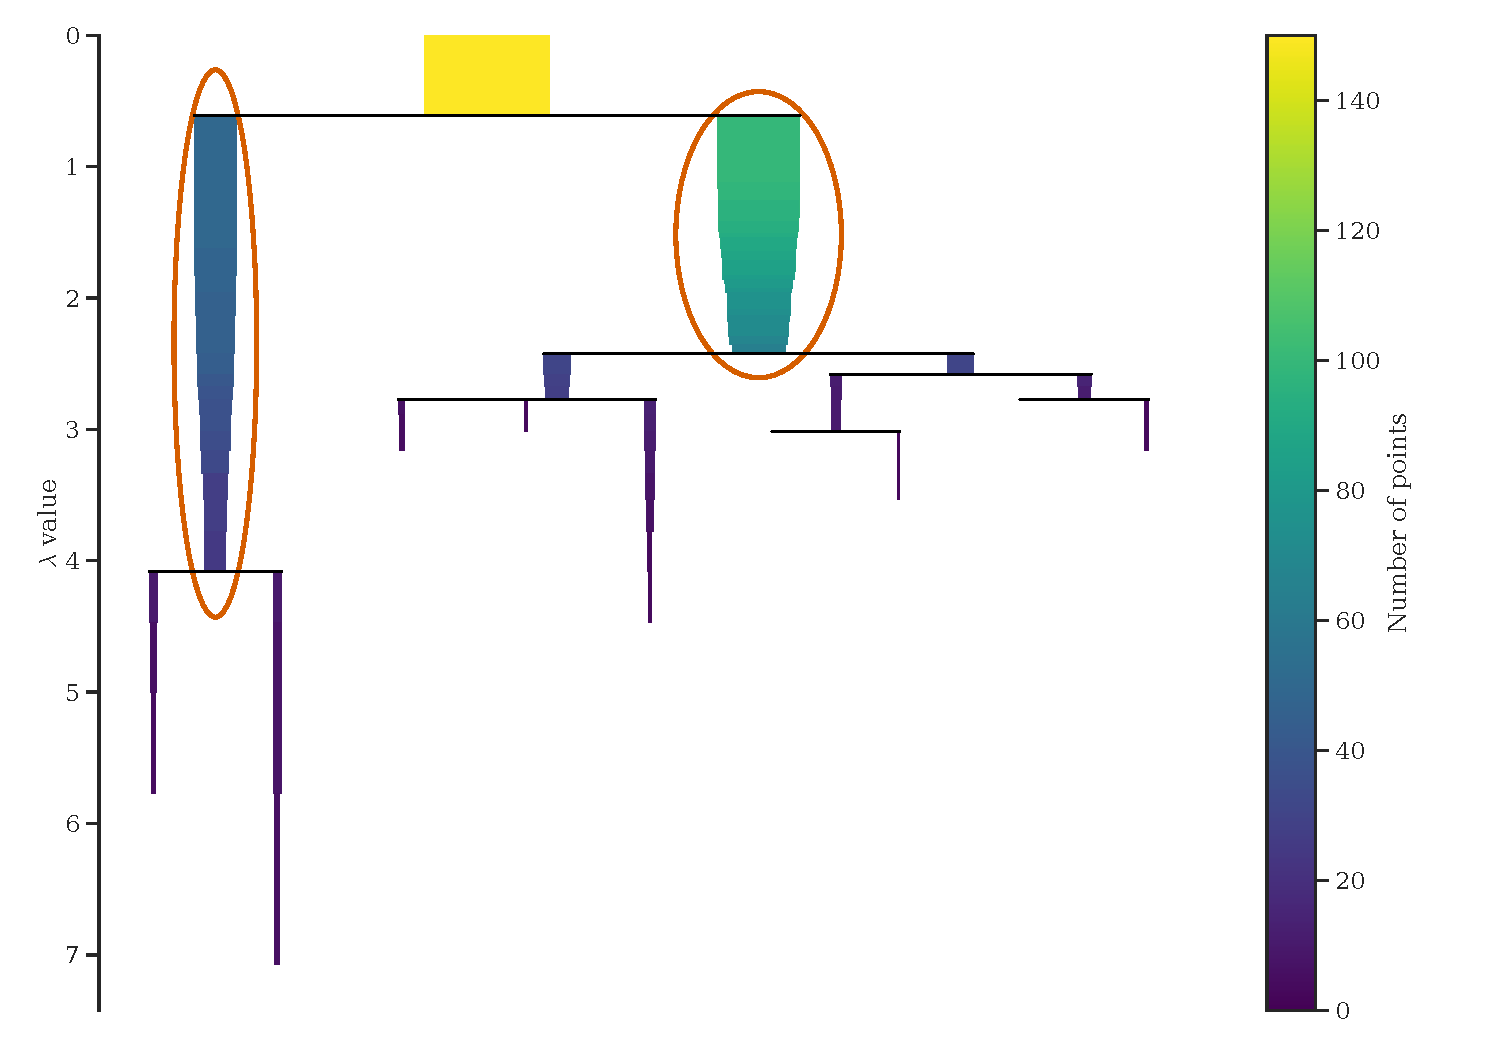
\includegraphics[width=10cm]{thesis/figures/hdbscan-condensed-tree-final-cut-example.pdf}
    \caption{Condensed dendrogram plot from HDBSCAN on the Iris data set \cite{Fisher1936}. The "final cut" is shown in the red circles. All data points below the circled clusters are considered noise.}
    \label{fig:hdbscan-condensed-dendrogram-final-cut-example}
\end{figure}

The main advantage of HDBSCAN is that is able to find the number of clusters automatically, can have differently shaped clusters and is able to mark data points as noise. Dealing with data points marked as noise can be a challenge, and depending on how one treats them (exclusion, each noisy data point in its own cluster, etc.), it may lead to very different results.

\subsection{ToMATo}
\label{sec:tomato-clustering}
Topological Mode Analysis Tool (ToMATo) \cite[2. ToMATo]{Oudot2015} is a clustering algorithm based on concepts from topological data analysis (TDA). In particular, ToMATo uses the concepts of persistence diagrams and prominence to perform clustering. The ToMATo clustering algorithm can be divided into three parts: density estimation and neighbour graph creation (1), mode-seeking (2) and merging (3). We refer to \cite[2. ToMATo]{Oudot2015} when explaining the algorithm.

First (1), any density estimation scheme is used in order to find dense areas in our data. A common choice is to use kernel density estimation with some kernel (e.g. gaussian). Let $\Tilde{f}(x_i)$ denote the estimated density of data point $x_i \in X, i = 1, 2, \ldots, n$. In addition to density estimation, a neighbourhood graph $G$ is computed in order to determine neighbours of data points. In the graph $G$, each vertex is a data point and edges represent neighbours. To compute $G$, it is common to use a $k$-nearest neighbour graph, where $k$ represents the number of neighbours.

Given the density estimator $\Tilde{f}$ and neighbourhood graph $G$, ToMATo uses mode-seeking (2) in order compute initial clusters. First, the vertices of $G$ are sorted by decreasing $\Tilde{f}$-value and iterated over. At each vertex $i$, compare the $\Tilde{f}$ values of vertex $i$ and its neighbours. If $\Tilde{f}(x_i)$ is greater than $\Tilde{f}$ of its neighbours, then vertex $i$ is denoted as a peak of $\Tilde{f}$. Otherwise, vertex $i$ is connected to the neighbour with the greatest  $\Tilde{f}$-value. By doing so, we create a spanning forest, where each spanning tree represent peaks of the underlying true density function. Given this spanning forest, the next step is to merge the trees to obtain a clustering.

The last step is the merging (3) of the spanning forest from (2). To do this, ToMATo iterates over the vertices of $G$ again (in the same order as in (2)) and a union-find data structure (denoted $\mathcal{U}$) is used to keep track of the merged spanning trees. The entries $e \in \mathcal{U}$ correspond to the union of spanning trees. The root of an entry $r(e)$, is the vertex in $e$ whose $\Tilde{f}$-value is the highest, i.e., a local peak of $\Tilde{f}$ in $G$. Now, iterating over the vertices of $G$, we check whether or not vertex $i$ is a peak of $\Tilde{f}$. If vertex $i$ is a peak of $\Tilde{f}$, i.e., root of some spanning tree $S$, a new entry $e$ is created in $\mathcal{U}$, in which $S$ is stored. The root of entry $e$ is set to the vertex itself, i.e., $r(e) = i$. If vertex $i$ is not a peak of $\Tilde{f}$, it means that it belongs to some existing entry $e_i \in \mathcal{U}$ and we look for potential merges of $e_i$ with other entries in $\mathcal{U}$. In particular, we iterate over neighbours $e \in \mathcal{E}$, $e \neq e_i$, of $i$ in $G$ and check whether $\min \enclc{ \Tilde{f}(x_{r(e)}), \Tilde{f}(x_{r(e_i)}) } < \Tilde{f}(x_i) + \tau$, where $\tau$ is the prominence threshold parameter. In other words, we check whether or not two entries have different $\Tilde{f}$-value and at least one of them has root with less than $\tau$ prominence. If this is true, $e$ and $e_i$ gets merged into a single entry in $\mathcal{U}$, i.e., $e \cup e_i$, and the entry with the lower root is merged into the one with the higher root.

Once the merging step is complete, we are left with a union-find structure $\mathcal{U}$. Every entry $e$ of $\mathcal{U}$ is connected to its parent entry $p(e)$ such that $\Tilde{f}(x_{p(e)}) > \Tilde{f}(x_e)$. In other words, by iteratively searching for the topmost parent, we can determine which cluster each entry (i.e. data point) is connected to. The ToMATo clustering algorithm can be seen as a combination of mode-seeking (from step (2)) and hierarchical clustering (from step (3)). As a result from the hierarchical structure, it is possible to visualize when entries in $\mathcal{U}$ gets merged into other entries, and thus, explain the lifespans of entries. More precisely, an entry in $\mathcal{U}$ is "born" when it is created in $\mathcal{U}$ and "dies" when it gets merged into another entry with higher root. Using persistence diagrams we can naturally explain the lifespans of entries and determine which entries live the longest (i.e. entries that never dies). The persistence diagram is also used to determine which value for $\tau$ we should use. Different values of $\tau$ results in different numbers of clusters. In practice, let $\tau = +\inf$ and use the persistence diagram of $\mathcal{U}$ to find a suitable threshold $\hat{\tau}$ such that the desired number of clusters is returned. Then, run ToMATo again using $\hat{\tau}$ as the threshold parameter to get the final clustering.

What is great about ToMATo is that it gives us a way to determine the numbers of clusters automatically (e.g. using some heuristic on the first persistence diagram to determine $\hat{\tau}$). In addition to this, ToMATo works with any metric, as long as a neighbourhood graph can be created using it (e.g. using Euclidean distance or similar metrics).

\subsection{Comparison of clustering algorithms}
In \cref{sec:clustering-algorithms}, we have described a number of algorithms for clustering data. We tabularize the strengths and weaknesses for each algorithm in \cref{table:clustering-algorithms-comparison}. Even though some algorithms might tick off more properties than others, it does not mean that it is a perfect algorithm for all types of data sets. In particular, one has to perform cluster validation to evaluate the results from various cluster algorithms to figure out what algorithm works the best. We explain how to validate results from cluster algorithms in \cref{sec:cluster-validation}.
\begin{table}[H]
    \centering
    \begin{tabular}{@{}lcccccccc@{}}
    \toprule
        & \multicolumn{8}{c}{Algorithm} \\ \cmidrule(l){2-9} 
        \multicolumn{1}{c}{Property} & \multicolumn{1}{l}{\rot{k-means}} & \multicolumn{1}{l}{\rot{MB k-means}} & \multicolumn{1}{l}{\rot{k-medoids}} & \multicolumn{1}{l}{\rot{GMMs}} & \multicolumn{1}{l}{\rot{Hierarchical}} & \multicolumn{1}{l}{\rot{Spectral}} & \multicolumn{1}{l}{\rot{HDBSCAN}} & \multicolumn{1}{l}{\rot{ToMATo}} \\ \midrule
        \trcolor Practical for large data sets & \xmark & \xmark & & \xmark & \xmark & & \xmark & \xmark \\
        Determining number of clusters automatically & & & & & \xmark & & \xmark & \xmark \\
        \trcolor Cluster centroids as data points & & & \xmark & & & & & \\
        Can have differently shaped clusters & & & & \xmark & \xmark & & \xmark & \xmark \\
        \trcolor Hierarchical clustering & & & & & \xmark & & \xmark & \\
        Robust against nosy data sets & & & \xmark & & & \xmark & \xmark & \xmark \\
        \trcolor Can identify noisy/anomalous data points & & & & & & & \xmark & \xmark \\
        User-defined distance metric & & & \xmark & & \xmark & \xmark & \xmark & \xmark \\ \bottomrule
    \end{tabular}
    \caption{Comparison of various properties for each clustering algorithm described in \cref{sec:clustering-algorithms}.}
    \label{table:clustering-algorithms-comparison}
\end{table}

\section{Cluster validation}
\label{sec:cluster-validation}
Given that we have performed clustering using some clustering algorithms, we now ask the question: which clustering algorithm performed the best on my data? Thankfully, there exist a handful of various methods designed for this task. In particular, we differentiate between internal and external cluster validation algorithms. Internal cluster validation algorithms assess the performance of the clustering using statistics of the data, without knowing the true labels at hand. External cluster validation algorithms, on the other hand, use the knowledge of the true labels. In this thesis, we will only use internal cluster validation algorithms, as we are mostly working with data where we do not know the labels beforehand. Recall that, in most clustering algorithms, we want the average distance between any two data points in the same cluster to be as small as possible (compactness); and the average distance between any two data points from different clusters to be as large as possible (separation). Internal cluster validation algorithms usually reflect compactness or separation of clusterings. In the next subsections, we will go over some common choices of internal cluster validation algorithms and discuss their strengths and weaknesses.

\subsection{Silhouette Coefficient}
\label{sec:silhouette-coefficient}
The Silhouette Coefficient is an internal cluster validation method which measures the goodness of clusterings \cite[p. 87]{Kaufman1990}. In particular, the Silhouette Coefficient measures how similar data points are to its own cluster (compactness) when compared to data points from other clusters (separation). The Silhouette Coefficient ranges from -1 to 1, where the best value is 1 and the worst value is -1. Values near 0 indicate that we have overlapping clusters (i.e. not well separated). This section is based on \cite[p. 87]{Kaufman1990}.

For any data point $x_i$ in the cluster $C_i$, the mean compactness $a(i)$ is defined as the average distance $d(i, j)$ between data point $i$ and all other data points in $C_i$, i.e., $j \in C_i, i \neq j$, as shown in \cref{eqn:silhouette-coef-a}.
\begin{align}
    a(i) = \frac{1}{|C_i| - 1} \sumlim{j \in C_i, i \neq j}{}{d(i, j)}
    \label{eqn:silhouette-coef-a}
\end{align}
where $|C_i|$ is the number of data points in cluster $C_i$. Smaller values of $a(i)$ indicate better compactness of clusters, and thus, better cluster assignments. Following, for any data point $x_i$ in the cluster $C_i$, the mean separation $b(i)$ is defined as the smallest distance from $i$ to any other cluster which $i$ does not belong, as shown in \cref{eqn:silhouette-coef-b}.
\begin{align}
    b(i) = \min_{k \neq i} \frac{1}{|C_k|} \sumlim{j \in C_k}{}{d(i, j)}
    \label{eqn:silhouette-coef-b}
\end{align}
Large values of $b(i)$ indicate that the clusters are well separated and that data points in $C_i$ are a good fit. Now, using the definitions of compactness and separation, the \textit{silhouette} of data point $i$ is defined as
\begin{align}
    s(i) = \begin{cases}
        \frac{b(i) - a(i)}{\max \enclp{a(i), b(i)}} & \mbox{if } |C_i| > 1 \\
        0 & \mbox{if } |C_i| = 1
    \end{cases}
\end{align}
Taking the average of all silhouettes $s(i)$, the mean Silhouette Coefficient is defined, as shown in \cref{eqn:silhouette-coef}.
\begin{align}
    SC = \frac{1}{n} \sumlim{i=1}{n}{s(i)}
    \label{eqn:silhouette-coef}
\end{align}
where $n$ is the number of data points in our data (e.g. $n$-dimensional data $X$).

The main advantages of mean Silhouette Coefficient are that it is simple, fast to compute and has a defined range from -1 to 1. The mean Silhouette Coefficient struggles with overlapping clusters (where $SC \approx 0$).

\subsection{Davies-Bouldin Index}
\label{sec:davies-bouldin-index}
The Davies-Bouldin Index (DBI) is an internal cluster validation method for evaluating results of clustering algorithms \cite{DaviesBouldin1979}. Similar to the Silhouette Coefficient, DBI measures the compactness and separation of clusters in order to measure the goodness of fit. This section is based on \cite{DaviesBouldin1979}.

To measure the compactness of a clusters, DBI introduces the notion of scatter within a cluster, denoted $S_i$. $S_i$ is computed by taking the mean of the sum of the distances to the cluster centroid of a given data point $i$, as shown in \cref{eqn:dbi-s}.
\begin{align}
    S_i = \enclp{ \frac{1}{|C_i|} \sumlim{x_j \in C_i}{} |x_j - \Tilde{C_i}|^p}^{1/p}
    \label{eqn:dbi-s}
\end{align}
where $C_i$ is the cluster associated to data point $i$, $|C_i|$ is the number of data points in cluster $C_i$, $\Tilde{C_i}$ is the centroid of cluster $C_i$ and $p$ denotes the power of the $L^p$ distance. A common choice is to set $p=2$, leading to Euclidean distances. A low value of $S_i$ indicate that the compactness of cluster $C_i$ is good. To compute the separation of clusters, DBI computes separation between clusters $C_i$ and $C_j$ by taking the distance between cluster centroids $\Tilde{C_i}$ and $\Tilde{C_j}$. We denote this cluster separation as $M_{i, j}$, as shown in \cref{eqn:dbi-m}.
\begin{align}
    M_{i, j} = ||\Tilde{C_i} - \Tilde{C_j}||_p
    \label{eqn:dbi-m}
\end{align}
where $p$ denotes the power of the $L^p$ distance. High values of $M_{i, j}$ indicate that the clusters are well separated. Combining the notion of cluster compactness $S_i$ and separation $M_{i, j}$, the measure of cluster goodness $R_{i, j}$ is defined, as shown in \cref{eqn:dbi-r}.
\begin{align}
    R_{i, j} = \frac{S_i + S_j}{M_{i, j}}
    \label{eqn:dbi-r}
\end{align}
In order to create a cluster measure that is symmetric and non-negative, $R_{i, j}$ was defined as such. Low values of $R_{i, j}$ indicate that we have compact and well separated clusters. For a given cluster $C_i$, DBI measures $R_{i, j}$ for all other clusters $C_j$, $j \neq i$, and uses the largest value of $R_{i, j}$, i.e., the worst-case scenario to compute the index. More formally, we define DBI in \cref{eqn:dbi}.
\begin{align}
    DBI = \frac{1}{n} \sumlim{i=1}{n} \max_{j \neq i} R_{i, j}
    \label{eqn:dbi}
\end{align}
where $n$ is the number of data points in our data (e.g. $n$-dimensional data $X$). The main advantage of DBI is the fact that is fast to compute and has a somewhat defined range (non-negative). Since DBI does not have any upper bound, it is more difficult to interpret the values, when compared to Silhouette Coefficient for instance.

\subsection{Caliński-Harabasz Index}
\label{sec:calinski-harabasz-index}
The Caliński-Harabasz Index (CHI) is an internal cluster validation method for evaluating clustering algorithms \cite{CalinskiHarabasz1974}. CHI measures compactness and separation of clusters in order to measure the goodness of fit for a given clustering. This section is based on \cite{CalinskiHarabasz1974}.

To measure the compactness of a clustering, CHI computes the sum-of-squares within cluster (SSW), as shown in \cref{eqn:chi-ssw}.
\begin{align}
    SSW = \sumlim{i=1}{n} ||x_i - \Tilde{C_i}||^2
    \label{eqn:chi-ssw}
\end{align}
where $n$ is the number of data points in our data, $x_i$ is the $i$th data point and $\Tilde{C_i}$ is the centroid of the cluster associated to $x_i$. Small values of SSW indicate that data points are compactly clustered. To measure the separation of clusters, CHI computes the sum-of-squares between clusters (SSB), as shown in \cref{eqn:chi-ssb}.
\begin{align}
    SSB = \sumlim{j=1}{k} |C_j| \cdot ||\Tilde{C_i} - \Bar{X}||^2
    \label{eqn:chi-ssb}
\end{align}
where $k$ is the number of clusters, $|C_j|$ is the number of data points in cluster $C_j$ and $\overline{X}$ is the center of all data points (i.e. mean). Large values of SSB indicate that the clusters are well separated. Following, the CHI is computed as the weighted ratio of SSB divided by SSW, as shown in \cref{eqn:chi}.
\begin{align}
    CHI = \frac{SSB}{SSW} \times \frac{n - k}{k - 1}
    \label{eqn:chi}
\end{align}
Since CHI is defined as the ratio between SSB and SSW, large values indicate better clustering. The main advantage of CHI is that it is fast to compute. Similar to Davies-Boundin Index, CHI is harder to interpret than Silhouette Coefficient for example, since the values are unbounded.

\section{Dimensionality reduction methods}
Working with data in high dimensions can be a difficult task at hand. Imagine that we have gathered some data, containing several features, and we would like to deepen our understanding of it. One approach we could do would be to visualize each feature by plotting them against each other, looking for bivariate relationships. Unfortunately, this is a rather cumbersome task and is hard to employ once a certain number of features is met (e.g. 10 features). Thankfully, dimensionality reduction methods can help us to reduce the dimensionality of data into some lower dimension where relevant properties of the original data are preserved. A typical application of dimensionality reduction methods is to lower the dimensionality to 2 or 3 such that one can visualize the data at ease. We will introduce two dimensionality reduction methods and explain how they work. In both subsections below, we assume that we are given some data $X \in \R^{n \times d}$ and that we want to reduce the dimensionality to some chosen hyperparameter $k$.

\subsection{Principal Component Analysis (PCA)}
\label{sec:pca}
Principal Component Analysis (PCA) is one of the most common dimensionality reduction metods \cite{Jolliffe2002}. PCA performs a linear mapping of the original data $X \in \R^{n \times d}$ to a (possibly) lower dimensional space $Y \in \R^{n \times k}$ ($k \leq d$) such that the variance is maximized in $Y$. One typically selects $k$ to a relatively low value, e.g., 2 or 3 if we would like to visualize the most varying part of the data or to a value such that a given variance threshold is met, e.g., explaining 90\% of the variance of the data. We refer to \cite{Jolliffe2002} when explaining PCA.

The PCA algorithm consists of several steps and we will go through them briefly. First, the mean of $X$ is computed, denoted $\overline{X} = \frac{1}{n} \sumlim{i=1}{n} x_i$, and subtracted from $X$, i.e., $X' = X - \overline{X} = \enclc{x'_1, x'_2, \ldots, x'_n}$. Next, the covariance matrix of $X'$ is computed, denoted $C \in \R^{d \times d}$, and the corresponding eigenvectors and eigenvalues of $C$ are computed, denoted $C_\text{eig} = \enclc{c_1, c_2, \ldots, c_d}$. Furthermore, the eigenvectors $C_\text{eig}$ are sorted by its corresponding eigenvalues in a descending manner. By doing so, we get a set of ordered eigenvectors such that the first eigenvector corresponds with the largest value, the second eigenvector corresponds with the second largest value and so forth. We denote this set of ordered eigenvectors as $C'_\text{eig} = \enclc{c'_1, c'_2, \ldots, c'_d}$. We then pick the $k$ first eigenvectors of $C'_\text{eig}$ and project the data onto them, essentially performing a change of basis. In addition to this, the mean of $X$ is added to complete the reconstruction, as shown in \cref{eqn:pca-projection}.
\begin{align}
    \label{eqn:pca-projection}
    Y = X' \trans{\begin{pmatrix}
    c'_1 & c'_2 & \ldots & c'_k
    \end{pmatrix}} + \overline{X}
\end{align}
The newly created matrix $Y = \enclc{y_1, y_2, \ldots, y_n}$ represents the original data $X$ in (a possibly) lower dimension $k$, such that the variance in the vectors are maximized. The vectors $\enclc{y_1, y_2, \ldots, y_n}$ are also referred to as principal components (PC), where PC1 is $y_1$, PC2 is $y_2$ and so forth.

\subsection{Uniform Manifold Approximation and Projection (UMAP)}
\label{sec:umap}
Uniform Manifold Approximation and Projection (UMAP) is a dimensionality reduction algorithm based on, among other things, ideas from topological data analysis \cite{2018arXivUMAP}. In particular, UMAP uses a fuzzy version of simplicial complexes in order to create a weighted graph representing the topological structure of the data in higher dimension. To explain how the fuzzy version works, we will illustrate with the example from the "How UMAP Works" documentation page \cite{how-umap-works-2018}.

Imagine that we are given some data from a noisy sine, $X = \enclc{x_1, x_2, \ldots, x_n} \in \R^{n \times d}$, as illustrated in \cref{fig:how_umap_works_raw_data}.
\begin{figure}[H]
    \centering
    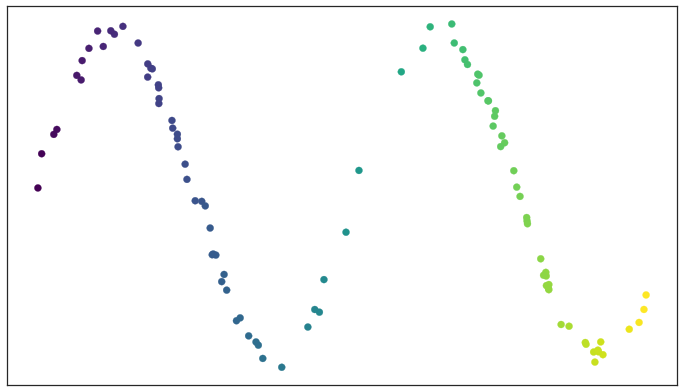
\includegraphics[width=10cm]{thesis/figures/how_umap_works_raw_data.png}
    \caption{Noisy sine wave (as illustrated by \cite{how-umap-works-2018}).}
    \label{fig:how_umap_works_raw_data}
\end{figure}

We would like to capture the topological structure of $X$, and we can do so by creating a simplicial complex built on $X$, illustrated in \cref{fig:how_umap_works_basic_graph}.
\begin{figure}[H]
    \centering
    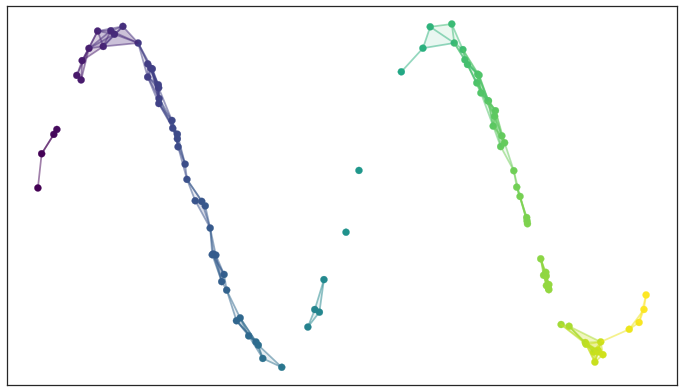
\includegraphics[width=10cm]{thesis/figures/how_umap_works_basic_graph.png}
    \caption{Simplicial complex built on a noisy sine wave (as illustrated by \cite{how-umap-works-2018}).}
    \label{fig:how_umap_works_basic_graph}
\end{figure}
We would like to capture the topological structure of all data points in $X$ and want a graph connecting all points. This, however is a problem, as there are some data points in \cref{fig:how_umap_works_basic_graph} which are disconnected from the simplicial complex, due to a small $\epsilon$ radius around each data point. In real word data, the data points are not uniformly distributed and selecting perfect $\epsilon$ to create a good simplicial complex is hard. The authors of UMAP overcome this problem by creating fuzzy open sets around each data point in order to create local connectivity in the graph, illustrated in \cref{fig:how_umap_works_umap_open_cover}.

\begin{figure}[H]
    \centering
    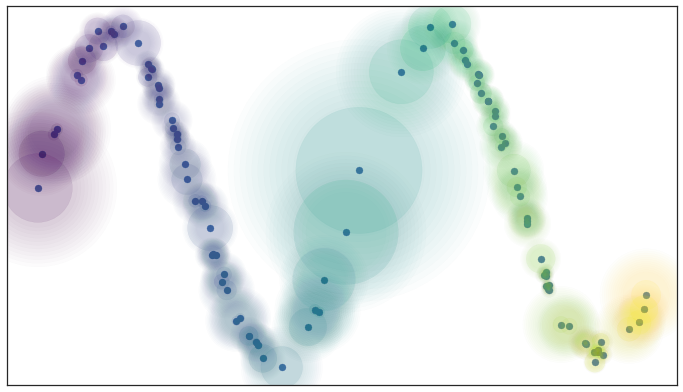
\includegraphics[width=10cm]{thesis/figures/how_umap_works_umap_open_cover.png}
    \caption{Fuzzy open sets around each data point of a noisy sine wave in order to create local connectivity (as illustrated by \cite{how-umap-works-2018}).}
    \label{fig:how_umap_works_umap_open_cover}
\end{figure}
To create the fuzzy open sets, the distance to the nearest neighbour of each data point is computed and the level of fuzziness decreases in terms of the distance beyond it, starting from 1 decreasing all the way to 0. If a data point has fuzziness level greater than zero, and edge is defined between the two data points, with fuzziness level as weight. We can also interpret the fuzziness level as the probability of the edge existing. We illustrate the connected graph in \cref{fig:how_umap_works_raw_graph}.

\begin{figure}[H]
    \centering
    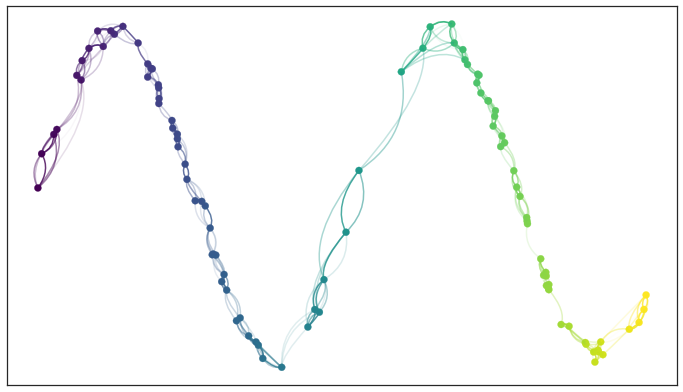
\includegraphics[width=10cm]{thesis/figures/how_umap_works_raw_graph.png}
    \caption{Connected graph where nodes are data points and edges between them are constructed given the fuzziness level between any two data point (as illustrated by \cite{how-umap-works-2018}).}
    \label{fig:how_umap_works_raw_graph}
\end{figure}
To finalize the connected graph from \cref{fig:how_umap_works_raw_graph}, the edges between any two data points gets converted into a single edge. We do this because we want the distance between two data points $a$ and $b$ to be the same; currently it depends locally on the distance to the nearest neighbour, as the fuzziness level decreases beyond it. To merge the edges between any two data points $a$ and $b$, the combined weight is computed by taking the union between them $w(a) + w(b) - w(a)w(b)$. This new combined weight is then used as weight of the single edge between $a$ and $b$. If we apply this process, unioning edges together, we end up with a fuzzy simplicial complex, illustrated in \cref{fig:how_umap_works_umap_graph}.

\begin{figure}[H]
    \centering
    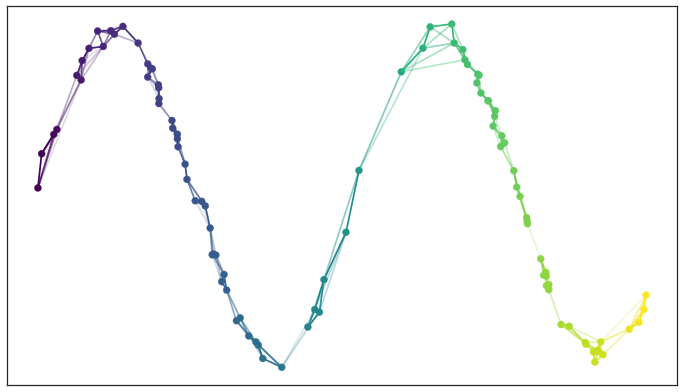
\includegraphics[width=10cm]{thesis/figures/how_umap_works_umap_graph.png}
    \caption{Fuzzy simplicial complex of some sine wave data (as illustrated by \cite{how-umap-works-2018}).}
    \label{fig:how_umap_works_umap_graph}
\end{figure}
Now, given the fuzzy simplicial complex of \cref{fig:how_umap_works_umap_graph}, we have a topological representation of $X$, capturing the topology of the manifold. We denote the set of all possible 1-simplices (i.e. edges) as $E$. The weight of a 1-simplex (i.e. edge) $e$ is computed using $w_h(e)$ in the high dimensional case. To get a good low dimensional representation of the high dimensional fuzzy simplicial complex, a low dimensional fuzzy simplicial complex is initialized and has weights denoted as $w_l(e)$ for edge $e$. To determine the weights $w_l(e)$, an iterative process is employed, where a loss function $L$ is optimized in a gradient descent fashion. Since we can interpret the weights of the 1-simplices of $E$ as probabilities of the edge existing (i.e. Bernoulli variables), the authors of UMAP uses cross-entropy as the loss function. More formally, the loss function $L$ is defined as
\begin{align}
    L = \sumlim{e \in E}{} \undertext{w_h(e) \log \enclp{\frac{w_h(e)}{w_l(e)}}}{Attractive force} + \undertext{(1 - w_h(e)) \log \enclp{\frac{1 - w_h(e)}{1 - w_l(e)}}}{Repulsive force}
    \label{eqn:umap-loss-function}
\end{align}

In the first term of \cref{eqn:umap-loss-function}, we have have an attractive force between the data points which $e$ spans, pulling them together; when $w_l(e)$ is large, the distance (i.e. weight) between any two data points becomes small. In the second term of \cref{eqn:umap-loss-function}, there is an opposite, repulsive force between the data points which $e$ spans, repelling them apart; when $w_h(e)$ is small (i.e. distance in high dimensional space), $w_l(e)$ will be small since we want to minimize the term. The process of pulling and repelling the weights makes the low dimensional representation of the data settle into a balanced state, such that it represents the high dimensional topological structure of the original data in a fairly accurate way. In practice, the UMAP algorithm uses a number of different tricks to optimize it, but we will not go into them here.

\section{Intrinsic dimension estimation}
In machine learning, the \textit{manifold hypothesis} states that in general, real-life high-dimensional data tends to live on a low-dimensional sub-manifold embedded within the high-dimensional space \cite[p. 16]{bengio2014representation}. In order to understand more about the underlying structure of the data we are working with, estimating the dimension of the low-dimensional sub-manifold can be seen as a viable strategy. The process of estimating the dimension of the low-dimensional sub-manifold is called \textit{intrinsic dimension (ID) estimation}. More generally, a $D$-dimensional data set $X \in \R^D$ is said to have an ID equal to $d$ if $X$ lies entirely within a $d$-dimensional subspace of $\R^D$ \cite{lee2015intrinsic}. Following, in this section we will introduce three methods for estimating the ID. For each of the methods described below, we assume that we have some data set $X \in \R^{n \times d}$ consisting of $n$ samples, where each sample is a $d$-dimensional vector. This section is based on \cite{lee2015intrinsic}, if not otherwise stated.

\subsection{Local PCA}
\label{sec:lpca}
One of the first and most simple kind of intrinsic dimension estimation algorithm is based on the PCA algorithm. By using the information gained from the eigenvalue decomposition of PCA, one can estimate the intrinsic dimension. This algorithm is referred to as the \textit{local PCA} (lPCA) method and was first introduced in \cite{Fukunaga1971}, which we refer to when explaining it.

The lPCA method works as follows. First, a sub-region around each data point $x_i \in X$, $0 \geq i \geq n$, is defined, either using radius or $k$-nearest neighbour ($k$-NN). For the sake of explanation, the the $k$-NN method is used, and we let $k$ denote the number of neighbours to include in the sub-region around $x_i$. The points in the sub-region around $x_i$ are denoted by $\text{N}_{x_i}$ ($x_i$ included in $\text{N}_{x_i}$). Furthermore, we run PCA on the data points $\text{N}_{x_i}$ and get the corresponding eigenvalues $\text{eig}\enclp{\text{N}_{x_i}}$. Using the computed eigenvalues, the lPCA method is able to identify the estimated ID by counting the number of eigenvalues that are greater than a portion of the largest eigenvalue. In other words, the estimated ID of data point $x_i$ using the lPCA method is defined as
\begin{align}
    \hat{d}_{x_i} = \sumlim{e \in \text{eig}\enclp{\text{N}_{x_i}}}{}{
        \begin{cases}
            1 & \mbox{if } e > \alpha \max \enclp{\text{eig}\enclp{\text{N}_{x_i}}} \\
            0 & \mbox{otherwise}
        \end{cases}
    },
    \label{eqn:lpca-esimated-id}
\end{align}
where $\alpha$ is a threshold parameter, determining how big of a portion an eigenvalue must be to be accounted for when estimating the ID. Typical values for $\alpha$ range between $0.01$ and $0.1$, as used by the experiments of \cite{Fukunaga1971}. The lPCA method can also estimate the ID of the whole data set $X$ by averaging $\hat{d}_{x_i}$ over all data points:
\begin{align}
    \hat{d}_{X} = \frac{1}{n} \sumlim{i=1}{n}{\hat{d}_{x_i}}
\end{align}
where $\hat{d}_{X}$ is the estimated ID of $X$.

\subsection{KNN}
A popular approach to estimate the ID is to use $k$-nearest neighbour ($k$-NN) graphs. In this subsection, we will explain a simplified version of the \textit{$k$-NN algorithm} for ID estimation, as explained by \cite[p. 651]{Carter2010}.

The $k$-NN algorithm starts by computing the total edge length of the $k$-NN graph built on the data $X$. Let $D(x_i, x_j)$ denote the distance between two data points $x_i, x_j \in X$, and let $\mathcal{N}_{k, i}$ denote the set of the $k$-nearest neighbours of data point $x_i$. Then, the total edge length of the $k$-NN graph is given by
\begin{align}
    L_{\gamma, k}(X) = \sumlim{i=1}{n} \sumlim{y \in \mathcal{N}_{k, i}}{} D(x_i, x_j)^\gamma,
    \label{eqn:k-nn-id-estimation-l}
\end{align}
where $\gamma>0$ is a constant, weighting the distances between the data points in the $k$-NN graph. For $\gamma>1$, big distances between data points become emphasized. Furthermore, assuming that the manifold hypothesis holds for the data $X$ (i.e. that the data $X$ can be fully described using a sub-manifold $X' \in \R^{n \times m}$), the equation \cref{eqn:k-nn-id-estimation-l} has an asymptotic behaviour \cite[Equation 2]{Carter2010} given by
\begin{align}
    L_{\gamma, k}(X) = n^{\alpha(m)}c + \epsilon_n
\end{align}
where $m$ is the unknown ID, $\alpha(m) = (m - \gamma)/m$, $c$ is a constant with respect to $\alpha(m)$ and $\epsilon_m$ is an error residual. In order to estimate the intrinsic dimension $\hat{m}$, a non-linear least squares approach is used; we will not go into detail of how it works here, but kindly refer the reader to \cite[p. 651]{Carter2010} for more details. The $k$-NN algorithm also uses sub-sampling of data in order to reduce noisy estimates of the ID. In particular, let $\enclc{p_1, p_2, \ldots, p_Q}$ be $Q$ integers such that $1 \leq p_1 < p_2 < \ldots < p_Q \leq n$. For each $p \in \enclc{p_1, p_2, \ldots, p_Q}$, sample $p$ data points from $X$, where the sampled data points are denoted $X_p^j$, for $j=1, 2, \ldots, p$. Let $L_p = \enclp{L_{\gamma, k}(X_p^1), \ldots, L_{\gamma, k}(X_p^p)}$. The estimated ID $\hat{m}$ is given by
\begin{align}
    \hat{m} = \argmin_{m \in \Z^{+}} \enclc{
        \min_c \sumlim{i=1}{Q} || L_{p_i} - {p_i}^{\alpha(m)}c\textbf{1} ||^2
    },
    \label{eqn:k-nn-id-estimation-m-hat}
\end{align}
where \textbf{1} is a vector of length $p_i$ consisting of all ones. By minimizing over both $c$ and $m$ in \cref{eqn:k-nn-id-estimation-m-hat}, this yields the estimated ID based on the $k$-NN graphs.

The described $k$-NN algorithm for estimating ID is a global estimator, meaning that estimates the ID of the whole data $X$. In order to estimate the ID locally for each data point $x_i \in X$, a similar approach that lPCA (\cref{sec:lpca}) uses can be applied. First, create a sub-region around $x_i$, denoted $\text{N}_{x_i}$, using $k$-nearest neighbours for instance. Then, apply the $k$-NN algorithm for estimating the ID on the $\text{N}_{x_i}$ sub-region in order to estimate the ID for data point $x_i$.

\subsection{TWO-NN}
Estimating the ID can be a hard task, especially if the underlying manifold of the data is twisted and curved. It is for this reason, the authors of \cite{Facco2017twonn} propose a two nearest neighbours estimator for ID estimation, called TWO-NN. TWO-NN uses the first and the second nearest neighbour of each data point in $X$ to estimate the ID. The authors claim that this minimality reduce the effect of complex manifolds, varying density and reduces the computational cost. We refer to \cite{Facco2017twonn} when explaining the algorithm.

The TWO-NN algorithm works as follows. First, the pairwise distances between every data point in $X$ is computed. For each data point $x_i$, we find the two shortest distances $r_1$ and $r_2$, where $r_2 \geq r_1$. Then, the ratio between $r_1$ and $r_2$ is computed, i.e. $\mu_i = r_2 / r_1$. Let $\mu = \enclp{\mu_1, \mu_2, \ldots, \mu_n}$. For data that comes from distributions with heavy tails, there is a high probability that $r_2$ is much larger than $r_1$, leading to large values for $\mu_i$, and thus makes the TWO-NN algorithm unstable. In order to cope with this, the authors of \cite{Facco2017twonn} suggest to remove the 10\% largest values of $\mu$ and only use the remaining 90\% for estimating the ID, leading to more stable results. We denote the discard fraction used to remove high values of $\mu$ as $\alpha=0.1$ and the remaining values for $\mu$ as $\mu^*$. The size of $\mu^*$ is computed as $n^* = n(1-\alpha)$. Following, we sort $\mu^*$ in ascending order, denoted $S(\mu^*)$, and compute the empirical cumulate as
\begin{align}
    F^{emp}(S(\mu^*)_i) = \frac{i}{n^*}.
\end{align}
The authors of \cite{Facco2017twonn} shows that the following relationship holds:
\begin{align}
    \frac{\log \enclp{1 - F^{emp}(S(\mu^*)_i)}}{\log \enclp{S(\mu^*)_i}} = d.
    \label{eqn:two-nn-id-equation-frac}
\end{align}
In order to estimate $d$ from \cref{eqn:two-nn-id-equation-frac}, linear regression is used. A linear regression model is trained on the data
\begin{align}
    \enclb{\undertext{\log \enclp{S(\mu^*)_i}}{x}, \undertext{-\log \enclp{1 - F^{emp}(S(\mu^*)_i)}}{y}},
\end{align}
where $i = 1, \ldots, n^*$. The slope of the computed linear regression model is the estimated ID, which we denote $\hat{d}$.

TODO: Write how to compute local ID estimates from TWO-NN model.

\subsection{MLE}
TODO \cite{Haro2008}.

\subsection{TLE}
TODO \cite{Amsaleg2019}.